\chapter{MECHANICAL SYSTEMS  DESIGN}

\label{Chapter3}




%Introduce your methods.
%Establish methodological connection. ..
%Introduce your instruments. ..
%Discuss your analysis. ...
%Provide background information. ...
%Discuss sampling process. ...
%Address research limitations.

\large{
\section{Wind Load Design}
\subsection{Introduction}
Engineers and astronomers are legitimately concerned about the effect of a wind load on a parabolic dish antenna and its structural elements when it is installed. Wind is the slow, horizontal movement of a mass of air from a high-pressure area to a low-pressure area on the outside of a closed structure.
Any structural design sensitive to uplift, shear, or lateral wind stresses is referred as having a wind load . As the height of the structure climbs, the load's amplitude grows, producing its impact. Stresses, material deformations, and structural displacements are caused by wind loads.
The weight of the building itself, often known as the permanent loads or dead load owing to gravity, is one of the many loads that can affect a building. But all permanent and transient structures are designed to withstand both structural and non-structural pressures. The intensity of a number of variables, including the size of the object—in this case, a wall or building—is used to calculate the wind load. A building must be able to withstand even the fiercest and most unusual gusts of wind. Hence, it is crucial to estimate the wind load before construction of any structural building begins.
The impact of wind is minimal and not a significant worry for the majority of residential buildings. The term "wind load" refers to the method for calculating the wind's impact on structural buildings.
In order to compute the wind load, it is an important procedure to first determine the surface area of the structure in the case of the parabolic dish antenna that will be impacted by the wind and how easily the wind travels over it (the drag coefficient).
The anticipated wind speed at the antenna's site is also an important factor to consider. These calculations may entail a substantial amount of mathematical analysis.


\subsection{Mauritian Cyclone Weather}


\subsection{Effects on wind loads on radio antenna structures}


The vibration of the telescope structure caused by unsteady wind on the telescope's mechanical structural system is one of the variables that can affect the performance of radio astronomy telescopes. It will be impossible to obtain the needed expected results if the terrain wind loading is not accurately estimated and characterised. When designing and building astronomical telescope structures, such as the tower and other supporting structures, the wind load is a significant consideration. Wind loads have a powerful effect on the telescope's application's efficiency as well as its safety.

%Evolution of telescope aperture diameter over the last four centuries, according to the trend by \cite{bely2003design} the diameter of the largest telescopes doubles about every 40 years.

Giant telescopes with diameters ranging from 10 to 305 metres have been the subject of various proposals in recent years\cite{bely2003design}. It is evident that the design of many future giant telescopes was successful and provided the necessary compliance to address structural-mechanism control interaction issues, among other things, by easily straightforwardly scaling up solutions that were more or less successful in building smaller or prototype-class telescopes.
Recent rapid development of a larger aperture diameter in the field of radio astronomy leads to more concerns about the impact of the wind load on the aperture and their structure towers. The evaluation of their safety and economic effectiveness will necessitates improved precision in antenna wind load computation. Accurate determination of the wind load on the reflector antenna during designing stage is crucial for limiting the impact of the wind on the surface deformation of the theoretically designed reflector and the entire antenna structure system \cite{elsbernd1983wind}. A reasonable wind-resistant design is essential to ensuring the structural system of an antenna function effectively. To ensure the safety and dependability of structures in wind-resistant design, the extreme wind load must be adequately evaluated. The extreme wind load is connected to the wind parameters and the aerodynamic properties of the structure.

Wind loading is a critical issue for both small and large telescopes and will be even more problematic for proposed future telescope designs like the SKA out- station in Mauritius. Wind loading on astronomical telescopes can be mitigated by embedding the telescopes in huge enclosures, such as domes, as and alternative to wind load test and calculations. An observatory dome may be defined as a structure that protects a telescope from the effects of wind and other external environmental conditions.
Before 1980, most observatories like the Haystack Observatory \cite{murga2016design}, the Onsala 20 m telescope\cite{rydbeck1977onsala, shaikh2019band} were designed to protect their telescopes from winds vibrations as much as possible by embedding the telescopes inside large domes with minimal openings. For many years, understanding the wind load within a telescope enclosure has been a source of worry according to  \cite{macmynowski2006wind}. Between the 1980s and 1990s, many studies by \cite{forbes1982wind,forbes1984large} were done to understand how air flowed through the telescope enclosures and the telescopes were able to withstand wind loading \cite{cho2003wind}.  Again, according to \cite{cho2003wind}, many studies have shed some light on issues of ventilation air flow through enclosures, but these studies did not produce data that was very useful for predicting the dynamic wind loading on the telescope.
Other studies have also attempted to measure wind pressure simultaneously at several points on a telescope primary mirror \cite{forbes1982wind,forbes1984large}, however the obtained information was limited \cite{cho2003wind}.
\cite{forbes1982wind} also conducted similar other studies to characterise the wind velocity at proposed and existing observatory sites such as Multiple Mirror Telescope (MMT) at Mt. Hopkins and at the United Kingdom Infrared Telescope (UKIRT). Another measurement by \cite{itoh1990mechanical} was made  at the Canada France Hawaii Telescope (CFHT) also with limited  spatial information.

In the study of \cite{perez2010telescope} mentioned that astronomical domes has a major source of poor vision since the domes are heated during the day and the warm air within the dome is maintained warm during the night. The warm air can only exit the dome through the slit that the telescope is looking through. This makes the cost of constructing and maintaining astronomical telescope domes extremely expensive, and do not entirely provide resistant  of wind load against telescopes. 

Wind power spectra have been  published for several sites \cite{hiriart2001wind}, \cite{forbes1982wind}, however the results vary somewhat in their behaviour from other sites. One of the key loads for astronomical telescope design is wind load on reflector surfaces, experts in this subject have proposed various techniques for calculating wind load, such as the Simiu method and the Kasperski method \cite{ye2021research}. Based on the basic theory of probability and a systematic analysis of the surrounding environment and turbulence, a random variable model for determining wind load has been developed. Extreme value analysis and computation design and installation theory are used to develop a numerical method  for calculating the maximum wind load that a structure can withstand.
It is important to estimate the required wind at the early stages of the design to influence the engineering of the telescope's structure and the control system \cite{macmynowski2006wind,odinets2018analysis}.


%................................................................................
%The team working on the current generation of large %telescopes in 1980s and 1990s did a number of studies to understand the effects of wind loading on telescopes \cite{cho2003wind}.Estimates of wind loads are required early in the design process, influencing the design of the telescope structures and control systems.
%In many cases, the main reason of transmission tower failure is the loading arising under
%off-design conditions due to the actions of High Intensity Winds (HIW).

%..............................................

\section{Wind Calculations Principles}

There are three recognised methods for determining the wind load of base station antennas according to \cite{bsi2005bs}, \cite{en19911} \cite{fournier2019recommendation} \cite{ kathrein_2016}, \cite{alliance2020recommendation} These methods are: 
\begin{enumerate}
    \item 
Numerical simulation of the wind flow
\item 
Wind tunnel testing 
\item
Calculation according to standards.
\end{enumerate}

\subsection{Numerical Simulations  Method}
% Numerical computations of wind flow is a software model engineering for prediction of wind flow of terrain over region of flow separation..
 
 A numerical simulation is a computer-based computation that uses a engineered software to create a mathematical model of a physical system. Most complex systems require numerical simulations to analyse their behaviour because their mathematical models are too complicated to give analytical solutions. With the fast advancement of computer technology,  computational Fluid Dynamics (CFD)  has grown in importance as a tool for product design using experimental fluid mechanics.\cite{kathrein_2016,en19911,omenzetter2000suppression,kim2000numerical,huawei_2017}
It allows for a more efficient and cost-effective product design process. However, due to the fluid's complexity, simulation alone is insufficient to compute the wind load, necessitating a significant number of wind tunnel tests.
 Figure \ref{fig:3.1} shows Numerical Computation simulation of Wind loading below.
 
 \begin{figure}[htp]
     \centering
 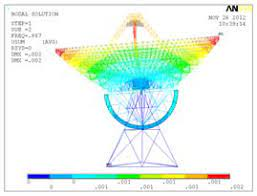
\includegraphics[width=4in]{Figures/Wind_load_ Displacement .jpg}
\caption{Computation Simulation of Wind Load:shows displacement of the Whole Structure under wind loading}
{\cite{liu2017reflector}}
     \label{fig:3.1}
 \end{figure}
 

 
\subsection{ Wind tunnel testing Method}

Wind tunnel experiments are used to forecast the wind loads and behaviours of a structure, structural components, and its walls under various wind conditions. The feedback for each standard provides detailed information on how the standards work and what they might be used for.
During wind tunnel tests, the model's aerodynamic forces and moments are directly monitored. The model is mounted in the tunnel using a specialised equipment called a force balance \cite{morris2010force}. The output of the balance is an indicator linked to the model's forces and moments. The Balance may be used to measure both lift and drag forces. The balance is calibrated against a known force value determined from the account of Reynolds number or Mach number drag impacts \cite{tienphuc2015numerical,gowen1953drag} on a model during testing, both before and periodically during the test. Data reduction or post-test processing are required for wind load force measurements. In predictive modelling, it's critical to always include the value of variables utilised in data reduction.
Figure \ref{fig:3.2} shows test set-up wind tunnel of parabolic antenna.

 
 
 \begin{figure}[htp]
     \centering
     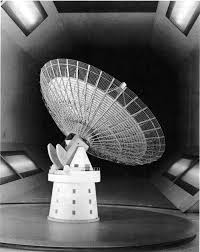
\includegraphics[width=3in]{Figures/wind_tunnel_test.png}
     \caption{Wind Tunnel Test Set-up of Parabolic Antenna}
     \cite{wyatt1964aerodynamics}
     \label{fig:3.2}
 \end{figure}
 
 
 
 

\subsection{ Calculation according to the standards Method}
The calculation according to standards or the generic formula is an accepted and reliable method or mathematical formula provided by some regulated bodies, such as the European standards EN 1991-1-4 \cite{en19911}, the American Society of Civil Engineers (ASCE) \cite{alinejad2020engineering}, the North American standard TIA-222-G \cite{rasool2021comparative}, and the Indian Standard IS:875 \cite{bhandari2011explanatory} released on wind load standards to determine the wind flow of terrain, influencing the design and operations of structures and structural elements. The wind load is calculated using the following generic formula:
\(F = A \times P \times C_d\)
\\
where F is the force or wind load\\
A is the projected area of the object \\
P is the wind pressure and\\
\(C_d\) is the drag coefficient \cite{kathrein_2016,huawei_2017}
According to a research by Kathrein \cite{kathrein_2016}, later wind tunnel experiments have revealed that the calculated conclusions are conservative rather than precise. This is why the data sheets are based on a combination of normal calculation and wind tunnel testing.


%\subsection{Principle of the Wind Load Determination}


%A big steerable antenna's support structure (including the feed structure) will often be made of an open framework with minimal solidity to reduce wind impacts. Unlike the previous part, which dealt with the paraboloidal reflector, these calculations deal with wind forces on tower and circular cylinder elements, which are frequently seen in support structures. Later, the effects of shielding between the reflector and the support structure will be addressed . The effects of solidity ratio, aspect or slenderness ratio, Reynolds number, the shapes of individual members (round, flat, angular, etc.) and, in the case of cylindrical members, the cross-sectional shape of the members are of primary interest in determining wind forces on these types of structures. Only at large levels of the solidity ratio does the influence of aspect ratio become significant. Particularly rounded and elliptical shapes, as well as geometries with rounded corners, are affected by the Reynolds number effect.

\section{Basic Wind Load Design}
In this chapter the assessment is carried out on the loads expected to carried by the antenna column and the dish through calculations according to the standard methods.
The wind load is calculated in compliance with the standard on the basis of a body with a circular cylinder tower and sphere parabolic reflector cross section. The resultant wind force and torque on a body enclosed in an up-draft can be represented in the following fashion using Bernoulli's principle and dimensional analysis theories.

\subsection{Wind Load is determined by the following formula:}



\begin{equation}
{F}_{W}={A_{eff}}.{q_p}.{C_d}.{{C_s}{C_d}} \label{eq:3.1}
\end{equation}
Where:

\begin{itemize}
\item \(F_W\) wind load
\item \(A_{eff}\) is projected Area
\item \(q_p\) is Peak velocity pressure
\item \(C_d\) is drag coefficient 
\item \( {{C}_{s}{C}}_{d} \) is structural factor for steel

\end{itemize}


\subsection{ Projected Area of the 2.4m parabolic reflector}

Figure \ref{fig:3.3} demonstrates the wind-loads and induced moments acting on a typical tracking antenna system referred to as axis angles. The a angels represent astronomical positions in elevation , \(\theta\), and azimuth, \(\psi\). The wind flow only in the horizontal direction is given by the angle, \(\psi\), which the wind makes with the plane of both the reflector side wall (the attack angle), is a function of the elevation and azimuth angles relative to the wind-speed, expressed by :

\begin{equation}
    \alpha = sin-^1 (\cos \theta \cos \psi)  \label{eq:3.2}
\end{equation}

\begin{figure}
    \centering
    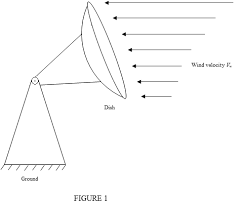
\includegraphics[width=3in]{Figures/wind_load_on_antenna.png}
    \caption{Block diagram of wind force on parabolic dish antenna }
    \cite{}
    \label{fig:3.3}
\end{figure}

The reflector depth-to-diameter ratio \(\frac{h}{d}\), surface solidity ratio \(\phi\), and surface geometry all affect the aerodynamic characteristics of parabola reflectors with sharp leading edges. The impacts of these factors on aerodynamics are shown in the following by calculating for offset parabolas with a diameter of 2.4m and evaluating lift and drag for fibber-glass reflector materials. Force coefficients are referenced to the plan-form area shown in equation \ref{eq:3.2}, and torque coefficients to the product of the plan-form area and diameter (rd3/4) in the case of the reflector. 

%****************(Wind loads are dynamic “force” placed by wind speed and its air density onto a building or structure. The force generated is a function of the wind speed,  the area offered by the antenna against wind, height of the structure and topographic of the region. )*********************

\begin{equation}
{A}_{{eff}} = {\pi}.\frac{d^2}{4} = {\pi}.\frac{{2.4}^2}{4} = 4.52m^2  \label{eq:3.3}
 \end{equation}
 
 %*******************************
%Torque =\(\frac{3^3}{4}\) 
%********************************


 \subsection{Wind load Characterisation}
 
 Different mechanisms might cause structural failure owing to wind loads. Over stressing occurs when peak stresses caused by relatively close wind loads surpass the material's endurance. Peak loads were analysed in the investigations that led to this approach, which provided a method for designing against over-stressing failure. When a material is continually loaded in a way that isn't as hard as it can withstand, fatigue failure can occur. 
 
The wind load dynamics of the area are the subject of our first fundamental investigation. The wind loads acting on the reflector and antenna support structure column surfaces shown in figure \ref{fig:3.3} were analysed using the Euro-code 1991-1-4 \cite {en19911} standard procedure. According to the Mauritius Meteorological Service data source, the strongest tropical cyclone recorded in Mauritius from 1931 and now had a characteristic 10 minute mean wind velocity at 10 metres above ground level of 184.2 km/h (3 seconds gust of 280 km/h) \cite{mms_2020}. The wind load data were obtained from the Mauritius Meteorological Service cyclone date \cite{mms_2020} and Coastal Land and Marine Solution (CLAMS) \cite{clams_2015}.
selecting and evaluating materials for steel structures. Given the site's location, the following environmental characteristics have been taken into account using the table's Euro-code 1991-1-4 \cite{en19911} of terrain category parameters in table \ref{Tab:3.1}.

\begin{table}[h]
\caption{Terrain category and terrain parameters}
\centering
\begin{tabular}{c r} 
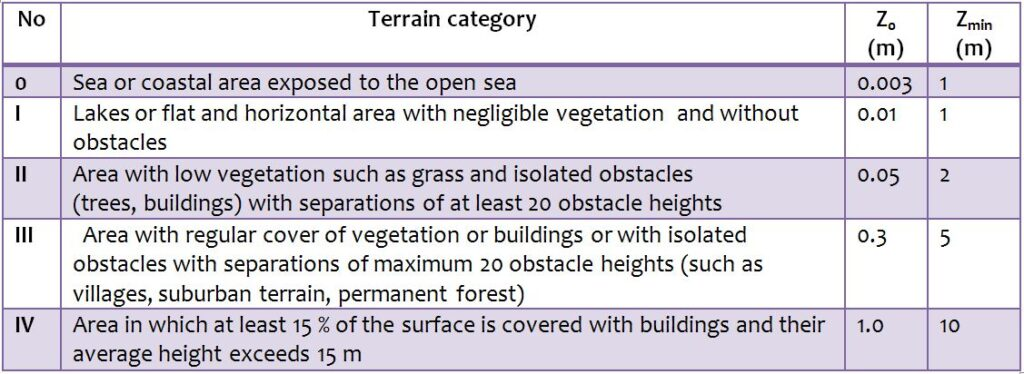
\includegraphics[width=5in]{Figures/Terrian_category.png} \label{Tab:3.1}\\
EN 1991-1-4 \cite{en19911}
\end{tabular}
\label{tab:hresult}
\end{table}

\subsection{The structural loads definition}

\textbf{Dead Load (DL)}\\
Dead loads, also known as permanent or static loads, are those that are built into a structure and remain throughout its lifespan. Table \ref{tab:3.2}  shows the vertical DL applied to the structure.



\begin{table}[h]
    \centering

  \caption{Vertical permanent loads information of the structure}
\begin{tabular}{ | p {7cm} | p {3cm} |}
    \hline
 The SPID BIG RAS-HR Rotor & 23kg\\ 
 \hline
 Parabolic dish & 86kg \\
\hline
 Dish brackets & 24kg\\
\hline
 Elevation motor adaptor rod & 10kg\\
\hline
 Counter weight and support&80g\\
\hline
 Feed and feed supports & 9.2kg\\
 \hline

    \end{tabular}
    \label{tab:3.2}
\end{table}



\textbf{Live Load (LL)}\\
Transient forces that travel through a structure or impact on any of its structural elements are referred to as live loads. Furniture, appliances, cars and other vehicles, and equipment are all examples of LL weights in residential building . For the purposes of this designs, this load is inapplicable.


\textbf{Environmental loads (EL)}\\
Because they're not inherently part of the structure and change over time, environmental loads are those ones may affect a structure based on its geography calculating location technically be termed active loads. Seismic activity, wind, rain, and snow are all referred to as EL.
With a reference to table \ref{Tab:3.1} antenna location is categorised under terrain category III as being an area with more than 15\% surface covered by trees.




\subsection {Drag coefficient is determined by the following formula:}

\begin{equation}
C_d = C_{f,0} . \psi_\lambda \label{eq:3.4} \\
= 2 \times0.8 = 1.6 
\end{equation}

\begin{itemize}[label={}]
\item Where:
 \item \(C_{f,0}\): force coefficient of cylinders without free-end flow is 0.8 (see Figure \ref{fig:3.4}) 
\item \(\psi_\lambda\) : end-effect factor (for length of the column is $<$ 15m,\(\psi_\lambda\) = 2)
\end{itemize}
   

\begin{figure}[htp]
    \centering
    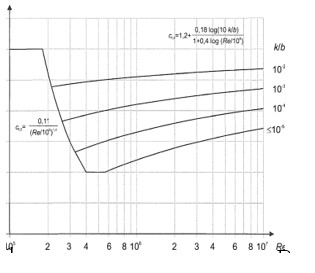
\includegraphics[width=3in]{Figures/CF2.jpg}
    \caption{Force coefficient Cf,O for circular cylinders without free-end flow}
    \cite{en19911}
    \label{fig:3.4}
\end{figure}



\subsection{Characteristic peak Velocity pressure is expressed by:}

\begin{equation}
q_p = 0.5 \rho \times V^2
\end{equation}

\begin{itemize}[label={}]
\item Where:
\item \(q_p\) is Characteristic peak Velocity pressure
\item  \(\rho \) : density of the fluid that’s passing the object
\item V is velocity of the fluid.(Characteristic 10 minutes mean wind velocity at 10 m above ground level at 184.2 km/h (3 seconds gust of 280kh/h) V = 64.3m/s \cite{cho2003wind,mms_2020}.
\end{itemize}

According to the EN \cite{en19911}, air density, which is dependent on the altitude, temperature, and barometric pressure to be expected in the region during a windstorm, should be obtained from the site location. As a result, for wind load assessments, we obtained our air density data from the nearest weather station, which is the MRT mini weather
meteorological station. Table \ref{tab:3.3} below shows the measured variable data from the MRT meteorological station.

\begin{table}[htp]
    \centering

  \caption{Meteorological data from MRT station on February 17th 2020}
\begin{tabular}{ | p {5cm} | p {4cm} |}
\hline
Date  of data collected & 17th February 2020 \\
    \hline
   Time of data collected   & 13hr 37min\\
    \hline
 Absolute pressure (P) &  \(1012 hPa \)\\ 
 \hline
 absolute temperature (T)  & 30.34 Kelvin \\
\hline
 \(R_{specific}\) T  &  287.058 J/(kg.K) \\
\hline

    \end{tabular}
    \label{tab:3.3}
\end{table}

\textbf{Density of air is define as:}

\begin{equation}
     \rho =\frac{P}{R}_{specific}T=\frac{{1}.{012} \times{{10}}^{5}}{{287}.{058}\times{303}.{49}} =1.246kg/m^3
\end{equation}

\textbf{The characteristic peak velocity pressure is then determine as:}
\begin{center}
    \( q_p  = 0.5 (1.246 \times {64.37}^2) = 5.162KN/m^2 \)
\end{center}
  
  
  
\subsection{Projected Area of the parabolic dish}

The reflector depth-to-diameter ratio (h/d), surface solidity ratio \(\phi\), and surface geometry together affect the aerodynamic characteristics of parabola reflectors with sharp leading edges. In the following, the effects of these parameters on the aerodynamics are indicated by calculating for offset parabolas with a diameter of 2.4m and measurements of lift and drag for fibber-glass materials used for the reflectors. Force coefficients are referenced to the plan-form area calculated in equation \ref{eq:3.3}.


%... yet to edit.
%To estimate wind pressure, we first use the peak factor method to calculate the highest value of the cyclone recorded coefficient under the whole wind direction and obtain the wind speed extreme value of the annual wind speed extreme series of the whole wind direction from the meteorological data and then take the calculated quantile value corresponding to a certain guarantee rate (return period) as the design wind speed extreme value. The influence of wind direction is not considered in the above calculation parameters.
% ...yet to


\textbf{Terrain Category IV}\\
Area in which at least 15\% of the surface is covered with buildings and their average height exceeds 15m Terrain category IV in table \ref{Tab:3.1} of the EN1991-1-4 \cite{en19911} table is applied. 


\subsection{Structural factor for steel} 

The structural load factor for a steel is a ratio of the theoretical design strength to the maximum load expected in service. The load factor is used in structural analysis to determine the design strength and compare it with maximum loads.


\textbf{ Structural factor for steel  is expressed by:}

\begin{equation}
    {C_S}{C_d} =\left(\frac{1+2k_pl_vZ_s\sqrt{B^2+R^2}}{1+7l_vZ_s}\right)
\end{equation}


\begin{itemize}[label={}]
\item {Where:}
\item \( {{C}_{s}{C}}_{d} \) is Structural factor for steel
\item \(l_v\) is turbulence intensity
\item \(B^2\) is background factor, allowing for the lack of full correction of the pressure on the structure surface 
\item \(R^2\) is  resonance response factor, allowing for turbulence in the resonance with the vibration mode
\item \(k_p\) is peak factor defined as the ratio of the maximum value of the fluctuating part of the response to its standard deviation of 1.66 on table C1 of the EN1991-1-1 \cite{en19911} 
\end{itemize}




\textbf{ Turbulence intensity might be determine first as:}
\begin{equation}
l_v(z) =  \frac{\sigma_v}{V_{m\left(z\right)}}
\end{equation}

Where:  \(V_m\) is the mean wind velocity at height z of 38.78m/s and \(\sigma_v\)  is the standard deviation of the turbulence 

\textbf{ Turbulence deviation also define as:}

\begin{equation}
\sigma_v = k_r . v_b. k_l\\
\end{equation}

Where: \(k_r\) is the terrain factor, \(v_b\) is the basic wind velocity of 51.17m/s and \(k_l\) is the turbulence factor with the recommended value for \(v_b\) is 1 given by \ref{Tab:3.1} of EN1991-1-4 \cite{en19911} on steel structures.
\begin{equation}
k_r = 0.19 {\frac{Z_0}{Z_{0,IV}}}^{0.07}
\end{equation}

\begin{itemize}[label={}]
    \item where:
\item \(Z_0\) is 1.0m, Roughness length for category IV given in table \ref{Tab:3.1} of EN1991-1-4.
\item \(Z_{0,IV}\) is 1.0m, Roughness length for terrain category IV given in table \ref{Tab:3.1} of EN1991-1-4.
\item \(Z_{min}\) is 10m, the minimum height for terrain category IV given in table \ref{Tab:3.1} of EN1991-1-4 .
\item \(Z_{max}\) is  200m, Terrain roughness from table 4.3.2 of the EN1991-1-4 \cite{en19911}
\end{itemize}

\textbf{Terrain factor is then expressed as:}
\begin{center}
    \(K_r = 0.19 {\frac{1}{1}}^{0.07} = 0.190\).
\end{center}


\textbf{Turbulence deviation now expressed as:}

\begin{center}
        \(\sigma_v = 0.19\times51.17\times1 = 9.722\)
\end{center}

\textbf{Turbulence intensity determined as:}

\begin{center}
    \(l_v(z) =  \frac{\sigma_V}{V_{m\left(z\right)}} =  \frac{9.722}{38.78}  =  0.25\)
\end{center}



\textbf{Background factor for the structure can be expressed by:}

\begin{equation}
B^2 = \frac{1}{1+0.9({\frac{b+h}{L_{z_s}})}^{0.63}}  = \frac{1}{1+0.9(0.928)} = 0.54
\end{equation}


\textbf{Resonance response factor can be define by:}

\begin{equation}
R^2 = \frac{\pi}{2.\delta} .S_L(z_s,\eta_{1,x}).R_h(\eta_h).R_b(\eta_b)
=\frac{\pi^2}{2\times0.05} \times 0.02(2.75\times0.405)\times(1.66\times0.405) = 1.47\\
\end{equation}

\textbf{Structural reference height of the column can be determined as:}

\begin{equation}
z_s = h_1 \plus \frac{h}{2} = 1.4 \plus \frac{2.4}{2} = 2.6m
\end{equation}

Where: diameter \textbf{\(h_1\)} of the dish  is given as 2.4m  and height \textbf{(h)} of the structure column is given as 1.4m.

\textbf{Structural factor of steel material is determined as:}
\begin{center}
    \({{C}_{s}{C}}_{d} = \frac{1+2.k_p.l_v\left(Z_s\right).\sqrt{B^2+R^2}}{1+7.l_v\left(Z_s\right)}  = \frac{1 + 2 \times 1.66 \times 0.25\times 2.6 \sqrt{{0.54}^2+{1.47}^2}}{1 + 7 \times0.25\times2.7}  = 0.95\)
\end{center}




\textbf{Wind Force acting on the structure is determine as:}

\begin{center}
    \({F}_{w} = 4.52 \times 5.162 \times 1.6 \times 0.95 = 35.564kN \)
\end{center}





\section{Antenna Column Design}

%Solidworks software was used for the design drawing and simulation of the antenna column or tower.
%Numerical calculation of tower compressive stress, bending stress, tower’s buckling and tower weight for safe load is calculated below.******************MOVE**********
    
 A variety of materials are used in the construction of structural buildings. Engineers must select the appropriate materials to ensure that buildings and structures are properly supported. A steel column is a vertical or tower structural element that provides crucial support in structure. They can support loads in compression or transfer loads to floors or foundations from beams, ceilings, floor slabs, or roof slabs. Near cross-section axes, steel columns may also carry bending moments. Steel is a widely used material for columns in building, despite the fact that there are many other options. It has a structure that is more durable, flexible, and stronger than concrete. Steel columns are also more lightweight and easier to build than concrete columns. The shape of circular columns is used to categorise them. There are more than four longitudinal steel bars that act as reinforcement bars within these columns. The bending resistance of circular columns is often higher than that of rectangular or square columns.
    
\subsubsection {Analytical Analysis}

Stress-strain relationships must be understood in order to determine the yield and strength of materials. Figure \ref{fig:3.5} shows the relationships that exist.
    
\begin{figure}[htp]
    \centering
    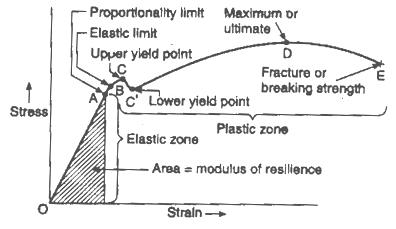
\includegraphics[width=3in]{Figures/Stress-Strain-Diagram.jpg}
    \caption{Stress- strain diagram}
    \cite{chaudhari_2015,sahin2016wind}
    \label{fig:3.5}
\end{figure}


Before beginning analytical analyses, it is necessary to mention the materials that have been chosen for the column. The material yield details for the 1.4-meter antenna column to be investigated on  a schedule 40 AISI 1020 mild Steel pipe with external and internal diameters of 273mm and 254mm under tensile vertical load of 35.56kN and 15.35kN moment of force.
  
 
\subsection{Axial Stress} 
 
  When a force acts perpendicular to a part of the body, it is known as axial stress as seen in figure \ref{fig:3.6}. This causes the column to fail by crushing or deforming in length at extremely high stress levels that transcend the column material's elastic limit.Axial stress is define define by the formula as:
  
  
  \begin{figure}[htp]
    \centering
    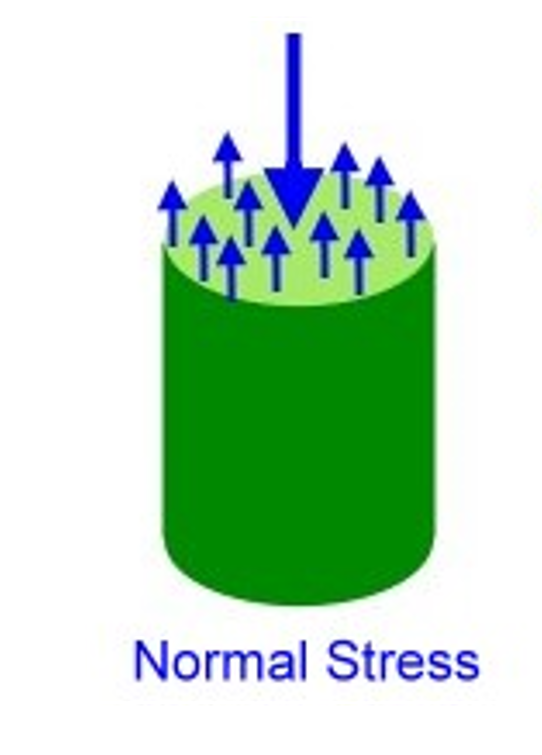
\includegraphics[width=2in]{Figures/Direct_shear_stress.png}
    \caption{Vertical column under axial load}
    \cite{amarine_2019}
    \label{fig:3.9}
\end{figure}
  
  
\begin{equation}
 \sigma a = \frac{P}{A}
\end{equation}
    
    \begin{itemize}[label={}]
\item where:
\item \( \sigma a\) is axial stress
\item A is the cross section area of the column
\item P is the tensile vertical load.
    \end{itemize}
    
\textbf{We first define the cross sectional  area  of the antenna Column as:}
    

\begin{figure}[htp]
    \centering
    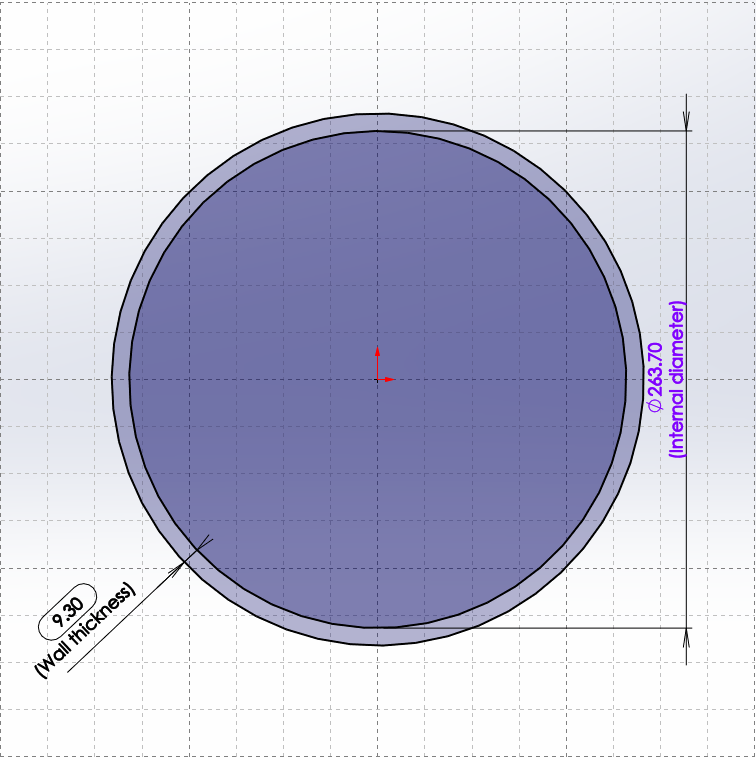
\includegraphics[width=3in]{Figures/Top_view_of_the_column.png}
    \caption{Top view of the column sketch}
    \label{fig:3.6}
\end{figure}

\begin{equation}
A = {\pi}\frac{{{ED}}^{2} - {{ID}}^{2}}{{4}}  = {\pi}\frac{{{0}.{273}}^{2} - {{0}.{263}}^{2}}{{4}}  = 0.000421{m}^{2}
\end{equation}

\begin{itemize}[label={}]
    \item where: 
    \item ID is the internal diameter of the hollow cylindrical cross section in figure \ref{fig:3.8}.
    \item ED is the external diameter of the hollow cylindrical cross section in figure \ref{fig:3.8}.

\end{itemize}

\textbf{Axial Stress is then determined as:}



\begin{center}
    \(\sigma a = \frac{{36000}}{{0.00768}} = 4.557MN/m\)
\end{center}


 \subsection{Bending Stress of the column} 
Bending stress is the typical stress that an object experiences when it is subjected to a heavy load at a specific spot, causing it to bend and fatigue. Figure \ref{fig:3.7} showed illustration of a bending stress on a member.
 
 \begin{figure}[htp]
    \centering
    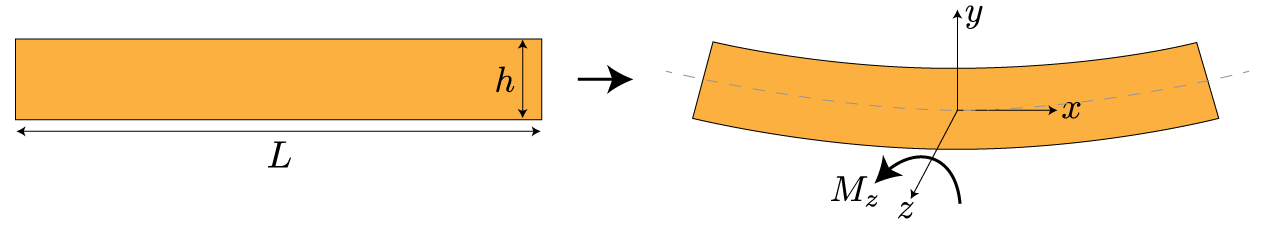
\includegraphics[width=3in]{Figures/bending_moment.jpg}
    \caption{Normal Stress in Bending}
    \cite{boston_2022}
    \label{fig:3.7}
\end{figure}
 
 \textbf{The column ending stress is determined in the following formula as:}
 
 \begin{equation}
\sigma b = \frac{M_y}{I}
\end{equation}

\begin{itemize}[label={}]
    \item \(\sigma b\) is the bending stress
    \item I is the moment of inertia 
    \item  M is the moment of force
    \item y is the vertical distance away from the neutral axis
\end{itemize}


\textbf{ As shown in Figure \ref{fig:3.6}, moment of inertia for hollow cylindrical cross section can be 
calculated by the following formula:}
\begin{equation}
    I= {\pi}\frac{{{ED}}^{{4}}-{{ID}}^{4}}{{64}} ={\pi}\frac{{0}.{273}^4-{0}.{263}^4}{{64}} = 0.0000378{m}^{4}
\end{equation}

\textbf{Moment of force is determined by the following formula as:}

\begin{equation}
M = {{F}\times{L}}
 = {15.35}\times{{10}}^{3}\times{1.4}= 21.5kNm 
\end{equation}



\textbf{also, vertical distance away from the neutral axis is expressed as:}
\begin{equation}
y = \frac{ED}{2}  =\frac{{0}.\mathbf{273}}{\mathbf{2}}= 0.1365m
\end{equation}

\textbf{Bending stress is define as:}

\(\sigma b = \frac{{M_y}}{{I}} = \frac{{23025}\times{0}.{1365}}{{0.0000378}} = 83.145MPa\) 





\subsection{Torsion Shear stress}


Torsion is the twisting of a structural member caused by torque. Torque causes rotation around the member's longitudinal axis. Figure \ref{fig:3.9} showed illustration of torsion in a vertical cylinder tube member.Whiles figure \ref{fig:3.10} also shows in circular shaft stress varies from the centre.
 
 \begin{figure}[htp]
    \centering
    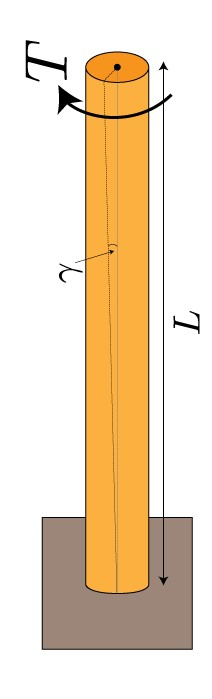
\includegraphics[width=0.7in]{Figures/torsion_shearstrain.jpg}
    \caption{Cylindrical tube element under torsion}
    \cite{boston_2022}
    \label{fig:3.9}
\end{figure}

\textbf{Torsion shear stress of a hollow tube can be expressed by the following formula:}

\begin{equation}
    \tau = \frac{M}{2A.t} = \frac{15.35}{2 \times 0.000421 \times 0.01} = 18.23MPa
\end{equation}



\begin{itemize}[label={}]
    \item where:
    \item \(\tau \) is the torsion
    \item M is the moment of force
    \item t is the thickness of the column (10mm)
    \item A is the cross section area
\end{itemize}


\begin{figure}[htp]
    \centering
    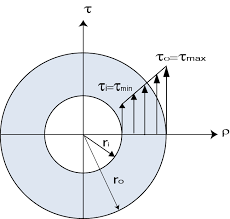
\includegraphics[width=3in]{Figures/Hallow_shaft.png}
    \caption{In circular shaft stress varies from the centre of torsion}
    \cite{bhandari2011explanatory}
    \label{fig:3.10}
\end{figure}



\subsection{Critical Load Buckling Strength }
Buckling is defined as "a sudden massive deformation of a structure due to a slight increase in an existing load under which the structure had shown little, if any, deformation earlier to the load being increased".  Column critical load buckling strength is determine as:

\begin{equation}
     P_{er} = \frac{\pi^2 .EI}{L^2} = \frac{\pi^2 \times 200 \times10^9 \times  0.0000378}{1.4^2} = 38.068MN
\end{equation}




\subsection{ Factor of safety  by soderbergs failure criteria }
The ability of a system's structural capability to be effective beyond its anticipated or actual loads is known as the factor of safety (FoS). An FoS is a constant value that a structure must satisfy or surpass according to the manufacture's legislation, specification, contract, or standard. It can be stated as a ratio that relates absolute strength to actual applied load.
Figure \ref{fig:3.11} shows the illustration of the Soderberg line, Soderberg line is a straight line joining \(S_e\) on the ordinate to \(S_{yt}\) on the abscissa is called the Soderberg line.  Goodman line is a straight line joining \(S_e\) on the ordinate to \(S_{ut}\) on the abscissa is called the Goodman line.

\begin{figure}[htp]
    \centering
    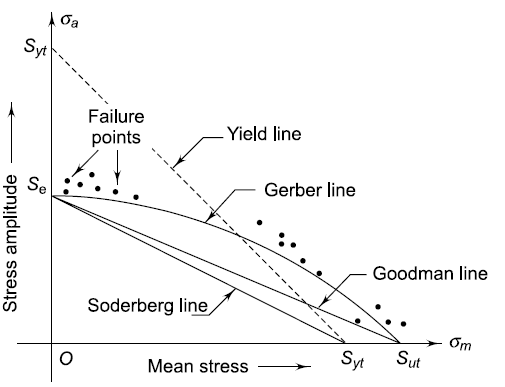
\includegraphics[width=3in]{Figures/soderberg&goodman_criteria.png}
    \caption{Gerber, Goodman, and Soderberg line}
    \cite{osakue2012linearized}
    \label{fig:3.11}
\end{figure}

\textbf{The column factor of Safety of the column is determined by the formula:}

\begin{equation}
 \frac {{1}}{{n}} = \frac{{\sigma a}}{{S_y}} + \frac{\sigma b}{S_e}
\end{equation}
 
 \begin{itemize}[label={}]
     \item where:
     \item \(S_e\) is the Endurance limit 
     \item \(S_y\) is the AISI 1020 Yield stress of 294.74MPa
     \item \(\sigma b\) is the bending stress
     \item \(\sigma a\) is the axial stress 
 \end{itemize}
 
 
\subsection{Endurance limit}
The endurance limit refers to the ultimate stress that a material can withstand for an indeterminate period of time. Although the criteria differ for different types of members and industries, it is usual practise to assume that holding a load for many million cycles of stress reversals suggests that the load may be carried indefinitely \cite{blodgett1964welded}.

\textbf{Endurance limit of the column is determined by the following formula:}
\begin{equation}
 (S_e) = K_a K_b K_c K_d K_e K_f {S_ e}^1
\end{equation}


\begin{itemize}[label={}]
    \item \(where:\)
    \item \(K_a\) is the surface factor 
    \item \(K_b\) is the size factor
    \item \(K_c\) is the  load factor of 1
    \item \(K_d\) is the load factor  of 1
    \item \(K_e\) is the reliability factor  of 1
    \item \(K_f\) is the miscellaneous factor of 1
    \item \({S_e}^1 = 0.5 {S}_{{ut}} = 0.5 \times 394.72 = 197.36MPa\)
     \item d is the diameter of the column
\end{itemize}


\textbf{Surface factor under endurance limit is determined as:} 

\begin{equation}
    K_a = a .{S}_{{UT}}^{b}
\end{equation}

\begin{itemize}[label={}]
    \item where:
    \item \(K_a\) is the surface factor
    \item a and b is hot rolled surface finish shown in table \ref{Tab:3.4}.
    \item UT is the AISI 1020 ultimate tensile stress of 394.72MPa
   
\end{itemize}


\begin{table}[htp]
\caption{Parameters for main surface modification factor}
\centering
\begin{tabular}{c r} 
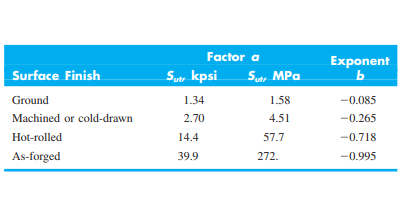
\includegraphics[width=5in]{Figures/surface_finish.png} \label{Tab:3.4}\\
\cite{horger1965metals}
\end{tabular}
\label{tab:hresult}
\end{table}

\textbf{Surface finish factor is expressed as:}
\begin{center}
    \(K_a = 57.7 \times {({394}.{72})}^{-{0.718}} = 0.788\)
\end{center}

    
\textbf{Size factor is also determined by the following formula from table \ref{Tab:3.5}:}

\begin{equation}
    K_b={1.51}d^{-0.157} = 1.51 \times 273^{-0.157} = 0.625
\end{equation}
  

\begin{table}[htp]
\caption{Modified Endurance Limit}
\centering
\begin{tabular}{c r} 
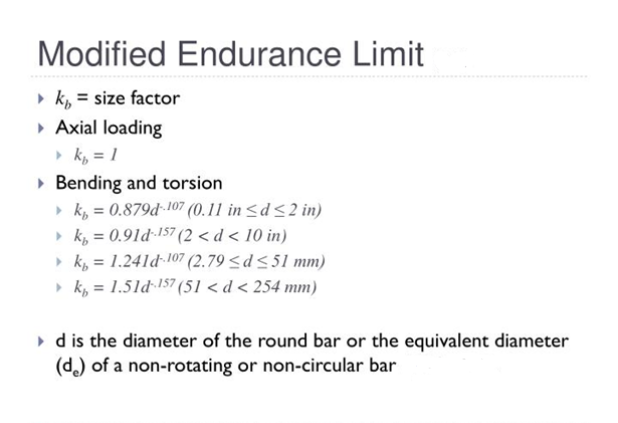
\includegraphics[width=4in]{Figures/Endurance_Limit.png} \label{Tab:3.5}\\
\cite{ncsu_2014}
\end{tabular}
\label{tab:hresult}
\end{table}




\textbf{Endurance limit is determined as:}
\begin{center}
     \(S_e = 0.788 \times 0.625 \times 197.36 = 97.199MPa\)
\end{center}

\textbf{ Factor of safety is expressed as: }

\begin{center}
    \(\frac{1}{n} = \frac{{3}.{255}\times{{10}}^{6}}{{97}.{199}\times{{10}}^{6}} + \frac{{47.049}\times{{10}}^{6}}{{294}.{74}\times{{10}}^{6}}\)  
\vspace{1cm} =  \(\frac{1}{0.342} = 5.178\)
\end{center}
The column design is therefore satisfactory.

\subsection{Column Deflection}
The degree to which a structural member can be displaced by a significant amount of load is defined as deflection. It's also known as the angle or the distance. The inclination of the deflected shape of the body under that load is directly related to the distance of deflection of a member under a load. Figure \ref{fig:3.12} shows the illustrations of Load-deflection diagram for column Buckling.

\begin{figure}[htp]
    \centering
    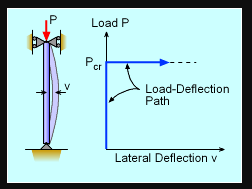
\includegraphics[width=3in]{Figures/column_deflection.png}
    \caption{Load-Deflection diagram for column buckling}
    \cite{kurt_2022}
    \label{fig:3.12}
\end{figure}
\textbf{Column load-deflection is determined by the following formula:}

\begin{equation}
 {D}_{f} = \frac{{F}{L}^{3}}{{3}{EI}} = \frac{{25000}\times {{1}.{4}}^{3}}{{3} \times{200}\times{{10}}^{9}\times{0}.{0000378}}  = 0.00302m
\end{equation}

\begin{itemize}[label={}]
    \item Where:
\item F is the tensile load 
\item L is the length of the column 
\item E is the Young’s Modulus of steel
\item I is the Moment of Inertia 
\end{itemize}
	
\subsubsection {Weight (W) of the 1.4m antenna column is determined as follows:}
\begin{equation}
W = (\frac{{\pi}}{{4}}({{ED}}^{2}-{{ID}}^{2})\times{d})\times h = (\frac{{\pi}}{{4}}({{0}.{273}}^{2}- {{0}.{263}}^{2})\times{7850}) \times 1.4  = 90.8Kg/m
\end{equation} 





\section{Antenna column base plate design}

A steel column structure's critical connection with a concrete foundation is represented by column base plate attachments. These column bases are often regarded to only be sensitive to axial compression and shear. To transfer the axial compressive force from the column to the foundation through the bedding material without exceeding the local bearing resistance of the foundation \cite{DesignofColumnBasePlates2010,punmia1998comprehensive}, the base plate should be thick enough, rigid enough, and strong enough.  The design procedure given by the guide are based primarily on the references given in America Institute of Steel Construction, INC. Steel guide 1 Base Plate and anchor rod design second edition \cite{fisher2006base} and design guide for Steel-to-Concrete Connection by \cite{cook1989design}. 


%The design guide justified in these Guides  are unique to this work.

This design guide provides minimum requirements for the design of connections between steel members and concrete. Design methods are presented for steel-to-concrete connections using cast-in-place anchors.
Figure \ref{fig:3.13} shows illustration of a typical Steel-to-Concrete Connection.


\begin{figure}[htp]
    \centering
    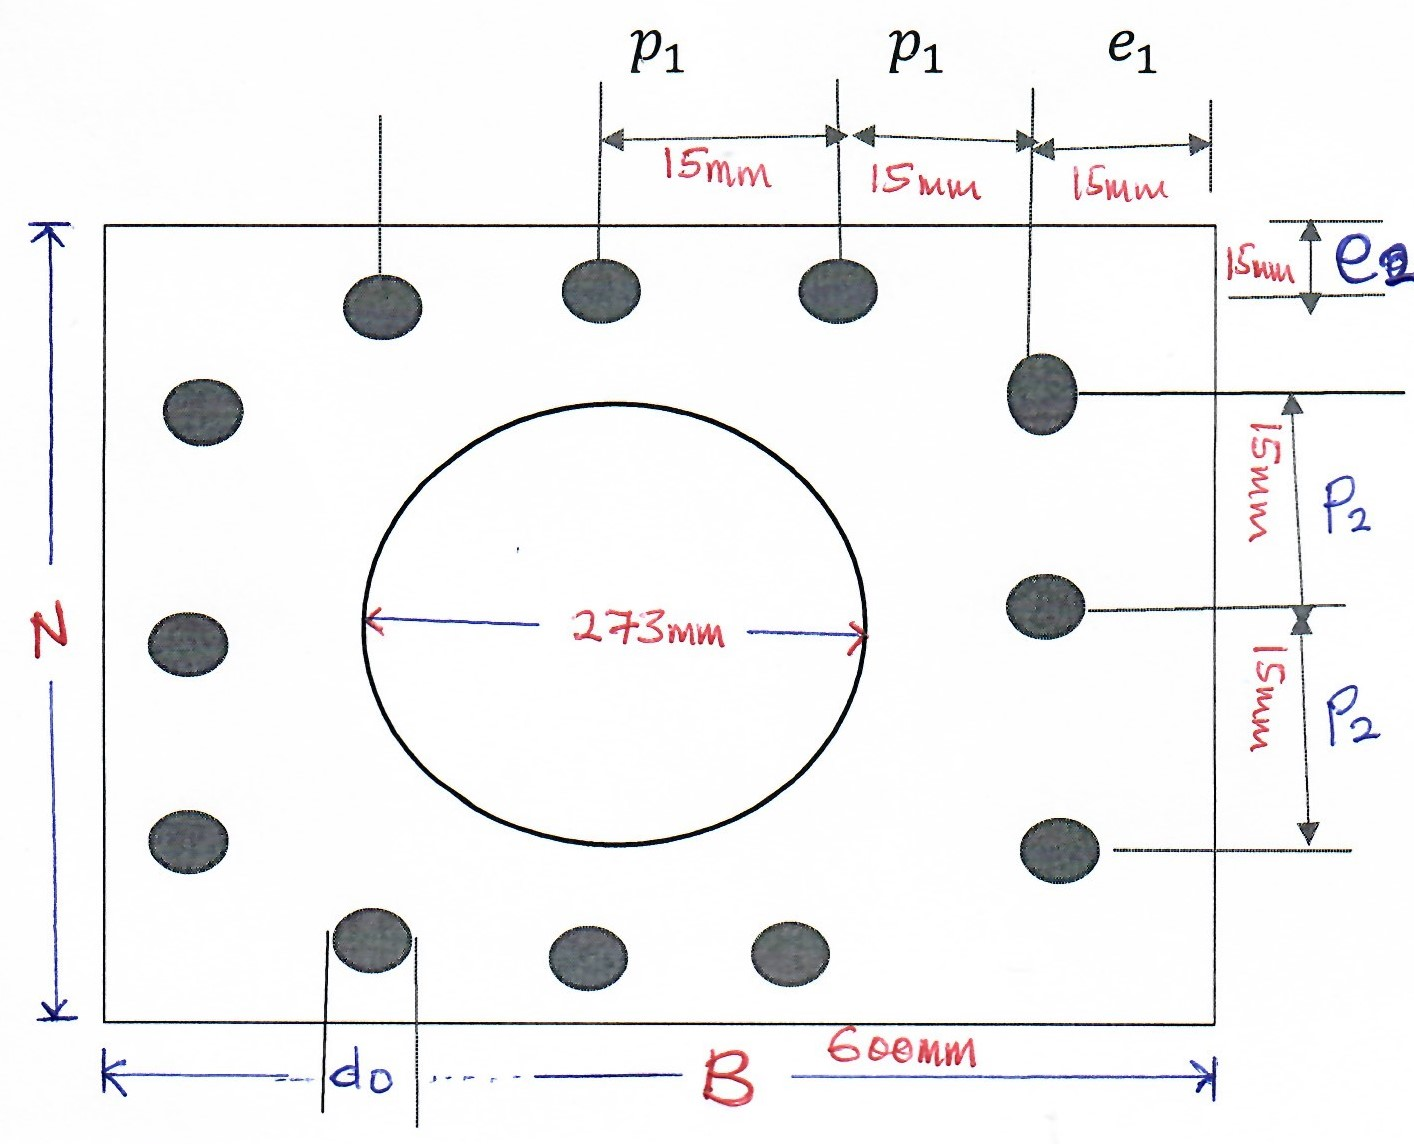
\includegraphics[width=3in]{Figures/base plate design.jpg}
    \caption{Steel-to-Concrete Connection}
    \label{fig:3.13}
\end{figure}



\subsection{ Base plate }

The following five design column load cases in column base plate connections were  followed in the designing of the  column base plate shown in figure \ref{fig:3.13}. 

\begin{itemize}
    
\item Determination of axial load and moment.
	
The base plate shall be of a sufficient thickness so that the design moment capacity per unit width of the base plate exceeds the maximum moment per unit width induced in the base plate by the tension- anchors \cite{cook1989design} 

\item  Base plate size selection, \({N \times B}\) 

\item Determine the equivalent eccentricity e = \(\frac{Mu}{Pu}\) and the critical eccentricity,

 If \(e_{crit}\), go to next step (design of the base plate with large moment)
 Check the inequality of the equation \(e_{crit}\) If it is not satisfied, choose larger plate dimensions.
 
\item Determine the equivalent bearing length, Y and tensile force in the anchor rod, Tu (LRFD), Ta (ASD).

\item  Determine the required minimum base plate thickness \(tp_{req}\) at bearing and tension interfaces. 
\end{itemize}


\textbf{Application of the design procedures as follows:}\\
A design analysis were performed on a base plate for an axial load of 25kPa and moments force of 15.35kN. Bending is about the strong axis for a CH40 wide flange column with diameter = 273mm and  \(b_{f}\) = 263mm specific minimum yield stress of steel base plate \({F_y}\) is 248.211MPa and the bearing stress between the plate and concrete \(f_{c}\) is 27.58MPa.


\begin{enumerate}[label={}]
\item {Where:}
\item Load Resistance Factor Design (LRFD) and Allowable Stress Design (ASD).
\item \(f_{p}\) is bearing stress between the plate and concrete.
 \item B is the base plate width.
 \item N is the base plate length.
\item \(F_{y}\) is specified minimum yield stress of steel base plate.
 \item \({t}_{p}\) is plate thickness.
 \item \({t}_{{p}({req})}\) is minimum plate thickness.
 \item \({b}_{f}\) is column flange width.
\item \(P_u\) and \(P_a\)  is required Axial compressive strength.
\item \(M_a\)  and \(M_u\)  is required bending moments strength.
\item  \({f}_{{p}({max})}\) is maximum concrete bearing stress.
\item   \( \phi\)  is the resistance factor .
\item  \( f_c \) is the minimum concrete compressive strength.
\end{enumerate}


\textbf{Case 1}\\

\textbf{ Determination of Required Axial compressive strength load and Required Bending Moments strength.}

\textbf{LRFD}
\begin{equation}
{P}_{u} = \phi P_l = (1.2 \times\mathbf{25}\times{\mathbf{10}}^\mathbf{3}) + (1.6 \times 2.28 \times 10^3) = 0.033 MPa/mm
\end{equation}



\begin{equation}
    {M}_{u}=  \phi P_l = 1.2 \times {15}.{35}\times{10}^{3} +  1.6 \times 83.145 \times 10^6 = 133.05MPa/mm
\end{equation}


\textbf{ ASD}

\begin{equation}
{P}_{a} = 25\times{{10}}^{3} + 2.28 \times 10^3
 = 0.0273MPa/mm
\end{equation}


\begin{equation}
{M}_{a}= 15.35\times 10^3 + 83.145 \times 10^6 = 98.495MPa/mm
\end{equation}



\textbf{Case. 2}\\ 

\textbf{Determination of axial load moment and Base plate size }

\textbf{LRFD}

\begin{equation}
A_{1}{req} = \frac{{P}_{u}}{{2} \phi {0.85}{f}_{c}} = \frac{0.033 \times 10^6}{2\times0.9\times0.85\times 27.58 \times10^6} = 0.0014 mm^2
\end{equation}



\textbf{ASD}

\begin{equation}
{A}_{\mathbf{1}{req}}= \frac{{\mathbf{\Omega}{P}}_a}{\mathbf{2}\times \mathbf{0}.\mathbf{85}{f}_{c}}= \frac{\mathbf{2}.\mathbf{5}\times\mathbf{25000}}{\mathbf{2}\times\mathbf{0}.\mathbf{85}\times\mathbf{27580000}} = 0.0013{{mm}}^{2}
\end{equation}

\textbf{Case 3}

\textbf{Optimisation of the base plate dimensions, N and B calculation}

\begin{equation}
\Delta = \frac{0.95d-0.85b_f}{2} =\frac{\left(0.95\times273\right)-(0.85\times263)}{2} = 17.9mm
\end{equation}

\begin{enumerate}[label={}]
    \item \({b}_{f}= 0.25446m\),
\item\(d= 0.273m\),
\item\(\phi\) = resistance factor for flexure 0.90,
\item \( \Omega\) = factor of safety for ASD 2.50 applied by the Occupational Safety and Health Administration (OSHA).
\end{enumerate}


\begin{equation}
    N =\sqrt{A_{1req}} + \Delta = \sqrt{0.0014} + 17.9 = 17.93mm^2 
\end{equation}


Therefore, N and B trial on 600mm or 0.6m

\begin{equation}
    A_{1} = N \times B = 600 \times 600 = 360000mm^2
\end{equation}


\begin{equation}
    A_2 = {4}{A_1} = 4\times360000 = 1440000mm^2
\end{equation}




\textbf{Case 4.}
\textbf{Determination of the eccentricity}


\textbf{LRFD}
\begin{equation}
    e = \frac{M_{u}}{P_{u}} = \frac{133.05}{0.033} = 44350mm
\end{equation}


\begin{equation}
    f_{pmax} = {\varphi}_{c} \times{0}.{85}{f}_{c}\sqrt \frac{A_{2}}{A_{1}} 
= 0.65 \times{0}.{85}\times27.58\times{{10}}^{6}\sqrt{\frac{360000}{1440000}} = 0.76MPa
\end{equation}

\begin{equation}
q_{max} = f_{pmax} \times{B} = 0.76 \times 10^6\times 600 = 456MPa/mm
\end{equation}

\begin{equation}
e_{crit}= \frac{N}{2}-\frac{P_{u}}{2q_{max}}  = \frac{600}{2}-\frac{0.033}{2\times 456} = 300mm
\end{equation}


 \textbf{\(e > {e}_{{crit}}\)} 
 
\textbf{ASD}

\begin{equation}
    e = \frac{M_{a}}{P_{a}} = \frac{98.495}{0.0273}  = 3607.87mm
\end{equation}



\begin{equation}
f_{pmax} = \frac{0.85f_c}{\Omega} \sqrt\frac{A_{2}}{A_{1}} = \frac{0.85\times27.58\times10^6}{2.5}\sqrt{\frac{360000}{1440000}} = 4.7MPa
\end{equation}

\begin{equation}
q_{max} = f_{pmax} \times B = 4.7 \times600 = 2820MPa/mm
\end{equation}

\begin{equation}
 e_{crit}= \frac{{N}}{{2}}-\frac{{P}_{a}}{{{2}{q}}_{{max}}} =\frac{600}{{2}}-\frac{{0.0273}}{{2}\times2820}= 300mm
\end{equation}

 \textbf{\(e > {e}_{{crit}}\) (3607.87 > 300}
 

From the above calculation the eccentricity, e, is greater than  \({e}_{crit}\); therefore, the design does not satisfy the the criteria under the condition case of a base plate with large moment must selected..



\textbf{Case 5.}

%\textbf{Verify bearing pressure from the bearing length}
%The anchor rod distance is 15mm

Determine e and \(e_crit\); check inequality in equation 3.4.4 to determine if a solution exists.


\begin{equation}
F = \frac{N}{2} - 15 = \frac{600}{2} - 15 = 285mm
\end{equation}

\begin{equation}
e_{crit} =    (f +\frac{N}{2})^2 = (285 + \frac{600}{2})^2 = 585mm
\end{equation}

\begin{equation}
   e = \frac{2P_u (e + f)}{q_max} =\frac {2 \times 0.033 (3607.87 +585)} {2820}= 49.39
\end{equation}

Since the \(e \leq e_crit \), therefore the inequality in Equations at case 4 is satisfied and a real solution for Y exists.




\textbf{Determining the bearing length, Y, and anchor rod tension, Tu or 
Ta}


\textbf{LRFD}

\begin{equation}
Y=\left(f+\frac{N}{2}\right)\pm\sqrt{\left(f +\frac{N}{2}\right)^2 - \left(\frac{2P_a[e+f}{q_{max}}\right)}
\end{equation}
\(= \left(285 +\frac{600}{2}\right)\pm \sqrt{285 +\frac{600} {2}^2-\frac{2\times 0.033 (44350+285)}{2820}}= 585 + 1.002 = 584mm\)

\begin{equation}
    T_u = q_{max}Y - P_u = 456 \times 10^6 \times 585 - 0.033\times 10^6 = 2.667MPa
\end{equation}



\textbf{ASD}

\begin{equation}
Y =\left(f +\frac{N}{2}\right)\pm \sqrt{\left[f + \frac{N}{2}\right]^2-\frac{2P_a(e+f)}{q_{max}}}
\end{equation}

\(=\left(285 +\frac{600)^2}{2}\right)\pm\sqrt{\left[285+\frac{600}{2}\right]^2-\frac{2\times0.0273(3607.87+285)}{2820}} = 585\pm 0.75 = 584mm \)

\begin{equation}
    T_a = q_{max}Y - P_a = 2820\times10^6 \times 584- 0.273\times10^6 = 1.64MPa
\end{equation}


\textbf{Case 6.}

\textbf{Determining the minimum Plate thickness at bearing interface.} 

\begin{equation}
m = \frac{{N}-{0}.{95}{d}}{{2}} = \frac{{600}-{0}.{95}\times{273}}{{2}}  = 170.3mm
\end{equation}



\textbf{Since the Y \( > \) m the minimum thickness of the base plate is determined as:}\\

\textbf{Determination of the bearing length Y}

 \textbf{LRFD}

\begin{equation}
{f}_{p} = (f_pmax) = 0.76MPa
\end{equation}

\textbf{ASD}

\begin{equation}
 f_p = f_(pmax)  = 4.7MPa/mm
\end{equation}



\textbf{LRFD}
\begin{equation}
t_{p(min)} = 1.5m\sqrt{\frac{f_{pmax}}{F_y}} = 1.5\times170.3\sqrt{\frac{0.076 \times10^6}{248.211\times 10^6}} = 4.47mm
\end{equation}


\textbf{ASD}

\begin{equation}
t_{p(min)} = 1.83m\sqrt{\frac{f_p}{F_y}} = 1.83\times170.3\sqrt{\frac{4.7\times 10^6}{248.211\times 10^6}} = 42.88mm
\end{equation}


\textbf{At tension interface:}

\begin{equation}
x=\frac{N}{2} -\frac{d}{2} = \frac{600}{2}- \frac{273}{2}= 163.5mm  
\end{equation}



\textbf{LRFD}

\begin{equation}
{t}_{{p}({req})} = 2.11 \sqrt{\frac{T_{U}x}{{BF}_{y}}} 
= 2.11 \sqrt{\frac{2.667\times 163.5}{600 \times248.211}} = 0.139mm
\end{equation}


\textbf{ASD}
\begin{equation}
{t}_{{p}({req})} = 2.58 \sqrt{\frac{T_{a}x}{{BF}_{y}}} 
= 2.58 \sqrt{\frac{1.64\times 163.5}{600 \times248.211}}
= 0.109mm     
\end{equation}


\textbf{Required plate thickness is determined using the value of n}

\begin{equation}
n=\frac{{B}-{0}.{8}{b}_{f}}{{2}}=\frac{{600}-{0}.{8}\times{263}}{{2}}=194.8mm
\end{equation}




 \textbf{ Required plate thickness is determined using the value of n calculated}
 
\begin{equation}
{t}_{{p}({req})} = 1.5n \sqrt{\frac{f_{p}}{{F}_{y}}} = 1.5 \times194.8\sqrt{\frac{4.7}{{248}.{211}}}= \frac{40.2}{2}mm = 20.1mm
\end{equation}
\textbf{control}
 The base plate thickness for the design 22mm, the nearest plate thickness available of 25mm is selected.


\textbf{ASD}
\begin{equation}
{t}_{{p}({req})} = 1.5n\sqrt{\frac{f_{p}}{{F}_{y}}} = 1.5 \times194.8\sqrt{\frac{4.7}{{248}.{211}}} = \frac{40.2}{2} = 20.1mm
\end{equation}
control




\section { Antenna Column Fabrication and Welding }
Welding is an important joining process in steel metal structure buildings and manufacturing.
After years of hard research, pioneering work by more forward-thinking engineers and builders, and a lot of documentation of findings and successes, welding has finally become universally regarded as a safe method to join structures. \cite{zaarour1996web}.

\subsection{Principles of Metal Arc Welding}
Welding is a combination two of  physical and chemical science .
The metal arc welding process generates heat by melting the parent metal material in the joint area using an electric arc. When the filler material melts and mixes with the parent metal material, it forms a molten weld pool.
The gas shielded method receive gas from a remote chamber, which is then delivered to the welding arc via the welding gun. The gas envelops the arc and basically seals it off from the rest of the world. The gas supply is managed by the the welding gun to keep it flowing at the required rate. Some methods use a flux that melts in the arc to create a slag layer that envelops and protects the weld pool during freezing. Slag hardens and releases on its own. The flux melts and generates a gas shield, which improves protection. The weld pool hardens as the welding progresses along the connection, bonding the parent metal material and welded metals together
The metal changes near the fusion line or fusion boundary when heat is applied to welds. This area of change is referred to as the "heat impacted zone.



 %Welding is the process by which two pieces of metal can be joined together. A welded joint is a permanent joint which is obtained by the fusion of the edges of the two parts to be joined together, with or without the application of pressure and a filler material \cite{khurmi2005textbook}. The process of welding does not merely bond the two pieces together as in brazing and soldering, but through the use of extreme heat and sometimes the addition of other metals or gases, causes the metallic structures of the two pieces to join together and become one \cite{TypesofWeldingProcesses2009}. Welding is largely used in fabrication as a substitute method for building or forging and as a replacement for bolted and riveted joints. It is also used for repairing broken and crack metals. 

\subsection{Types of Welded Joints}
 Generally, there are five recognised types of welding joints, according to the American Welding Society: Butt, Corner, Lap, Tee, and edge joint. Illustration of welding joints shown in figure \ref{fig:3.13}


\begin{figure}[htp]
    \centering
    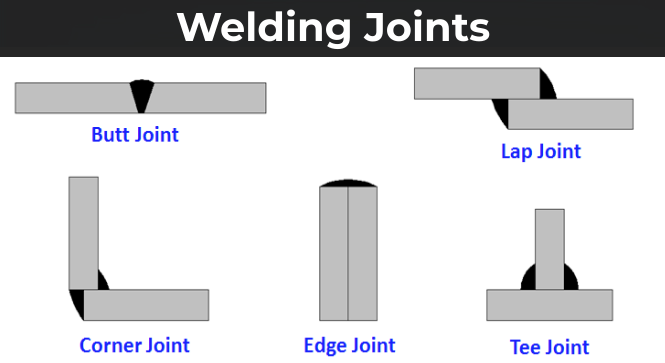
\includegraphics[width=4in]{Figures/welding-joints-types.png}
    \caption{The five types of welding joints}
    \cite{tvm@2017_2017}
    \label{fig:3.13}
\end{figure}

\subsection{Typical weld in a tubular tower}
The two most common types of welds are the fillet weld and the groove weld. Fillet weld examples include lap joint – fillet welds placed in the corner formed by two plates and tee joint – fillet welds placed at the intersection of two plates. Groove welds, on the other hand, consist of deposits in a gap or groove between two parts to be connected. Examples of groove welds are butt, tee, and corner joints with bevelled (prepared) edges. The illustrations of typical fillet and butt welds terminology used in welding connections shown in figure \ref{fig:3.14}.

\begin{figure}[htp]
    \centering
    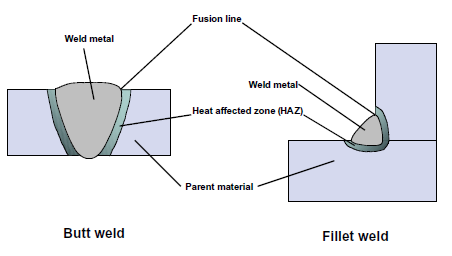
\includegraphics[width=4in]{Figures/Terminology_welding.png}
    \caption{Typical weld details in a tubular tower Butt and Filet weld between two metals}
    \cite{steel_2016}
    \label{fig:3.14}
\end{figure}

\subsection{Antenna Column Base-plate welding parameters}
During its lifetime, a structure made of steel is subjected to constant loads like wind and waves. There will be a few little cracks as a result of these constant loads. Daily expansion of these fissures could eventually cause a collapse. As a result, calculations for fatigue as well as buckling must be made while designing the tower. In sectors like welding or flanges, fatigue is crucial. The number of cycles and the stress interval are two critical elements for fatigue. Selecting the most appropriate joint type and weld type is central to successful engineering and manufacturing. Base metal preparation, joint access, weld distortion, overall strength, fatigue performance, and corrosion resistance are a few examples of connected qualities that must abide by the safety and service criteria for the application in which they are employed.The following design calculations and analysis were carried out for the welding of the antenna column base plate.


\subsection{Circular fillet weld}
When two circular shafts, pipes plates are joined together at an angle or perpendicularly, it is known as "fillet welding". The typical application of circular fillet welds in torsion is shown in Figure \ref{fig:3.16}. The weld is loaded in shear for this loading application, same like the longitudinal weld loaded in direct tension.



\begin{figure}%
    \centering
    \subfloat[\centering Circular fillet weld with torsional loading] 
    {{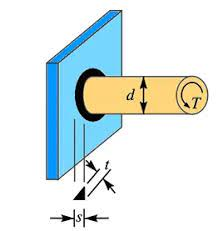
\includegraphics[width=4cm]{Figures/circular_fillet_weld.jpg} }}%
     \cite{Dannana2021How}
    \qquad
    \subfloat[\centering Circular fillet weld with axial loading]{{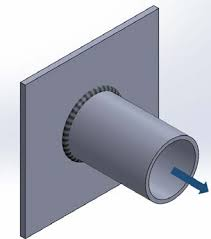
\includegraphics[width=3cm]{Figures/circular_fillet_weld_axial.jpg} }}%
    \cite{doane_2016}
    \caption{Circular Fillet Weld}%
    \label{fig:3.16}%
\end{figure}


\subsection{Bending stress in circular tube fillet weld}



\textbf{Bending stress of the column weld joint is determined by the following formula}

\begin{equation}
\sigma b = \frac{P_b {\times L} {\times r}} {I} = \cfrac{15350 {\times 1.4} {\times 0.273}} {\pi ( 0.273^4 - 0.253^4)} = 1.28MPa
\end{equation}



\begin{enumerate}[label={}]
\item where:
\item \(\sigma b\) is bending moment at the section in question
\item I is moment of inertia of the section,
\item L is distance from neutral axis to the point at which stress is desired in. = 1.4m
\item\({P}_{b}\) is bending stress = 15.35KN
\item  Diameter of tube(d) = 273mm
\item Radius of tube (r )= 0.273m
\item Size (or leg) of weld (s)  = 70mm 
\item  minimum throat width of fillet weld (t) = 0.707mm 
\item Moment of force \(P_b\) = 35.56KN  (Reference from wind load determination in equation \ref{eq:3.1})
\end{enumerate}


\subsection{Shear and Torsion loading in the welded fillet joint}

The case of shear and torsion loading will be taken into consideration and as shown in Figure \ref{fig:3.16}(a). The dynamic approach, which is more conservative, will be employed for this section to determine the required weld strength for these connections. The ultimate strength method can also be used.


\textbf{Primary shear and torsion loading in the welded fillet joint is expressed in the following formula: } 
\centering
\begin{equation}
\tau_1 = \frac{F}{A} =\frac{P_b}{A}=\frac{15350}{1.414\times\pi\times s\times r} =\frac{15350}{1.414\times\pi\times70\times0.273} = 0.16KPa
\end{equation}

\textbf{Secondary shear and torsion loading in the welded Fillet joint is expressed in the following formula: }
\centering
\begin{equation}
\tau_2 = \frac{{M}_{r}}{{Z}} = \frac{{P}_{{b}}\times{L}\times{r}}{{0}.{707}\times{\pi}\times{s}\times {r}^{3}} = \frac{{35560}\times{1}.{4}\times{0}.{273}}{{0}.{707}\times{\pi}\times{70}\times{{0}.{273}}^{3}} = 0.4296KPa 
\end{equation}

\textbf{where: Section modulus of the weld section  \(Z = \pi. t.s.d^3\)} 

 \textbf{The resultant torsion shear stress at the welded joint is determined by:}
\centering
\begin{equation}
\tau_{total} =\sqrt{{\tau_1}^2 + {\tau_2}^2} = \sqrt{{ 0.16}^2+{0.4296}^2} = 0.345KPa
\end{equation}




\subsection{Shear and bending loading in welded joints}



\textbf{Primary Shear and bending loading in welded joints is determined by the formula }
\centering
\begin{equation}
\tau_1=\frac{K_fs P_b}{A}   = \frac{2.7\times 15350}{ 1.414\times\pi \times 70 \times 0.273} = 0.488KPa
\end{equation}

\textbf{Secondary shear and bending loading in welded joints is determined in the following formula}
\centering
\begin{equation}
\tau_2 = \frac{{M}_{r}}{{I}} =\frac{{P}_{{b} }\times{L}\times{r}}{{I}} = \frac{P_b \times L \times r} {0.707 \times{\pi}\times{S}\times{r}^\mathbf{3}} =\frac{35560 \times 1.4\times 0.273}{0.707 \times \pi \times 70 \times 0.273^3 } = 4.296KPa
\end{equation}


\textbf{The  maximum stress of the welded joint is determine by the following formula}

  \begin{equation}
    \tau_{total} =\sqrt{{\tau_1}^2+{\tau_2}^2} =\sqrt{{0.488}^2+{4.296}^2} = 18.943KPa
  \end{equation}
 

\textbf{Allowable Shear stress of the weld joint is determined from the formula:}

\begin{equation}
{\tau}_{{all}} = 0.4{S}_{y} =  0.4 \times 294 \times{10}^6 = 117.6MPa
\end{equation}

\begin{enumerate}[label={}]
\item Where: Yield strength \(S_y\) of the material is 294.74MPa
 \end{enumerate}
 
 From the calculations above since the \({\tau}_{{all}}\) is greater than  \({\tau}_{{total}}\) \((294.74MPa \geq 18.943KPa\)), therefore the designed welded joint is satisfactory.
 



 
\subsection{Fatigue Stress of the weld joint}

In a process known as fatigue, materials that are subjected to cyclic loads that are much below their material's failure stress under normal conditions may initially show deformation that will eventually spread and result in the component failing.

\textbf{Fatigue stress of the weld joint is expressed in the formula as:}

\begin{equation}
 {n}_{f}=\frac{{S}_{{se}}}{{\tau}_{{total}}} = \frac{{97}.{199}}{18.943} = 5.131MPa
\end{equation}


\subsection{Factor of Safety for Weld Joint }
The ability of a system's structural capability to remain stable beyond its anticipated or actual loads is known as the factor of safety (FoS). FoS of the weld joint is expressed in the formula as follows:

\begin{equation}
n=\frac{0.577\times S_y}{\tau_{total}} = \frac{0.577\times294.74\times{10}^6}{18.943\times{10}^3} = 8.97\times 10^9
\end{equation}

\(n=\frac{0.577\times S_y}{\tau_{total}} = \frac{0.577\times294.74\times{10}^6}{18.943\times{10}^3} = 8.97\)

Since \(n \geq n_d\), that is \(8.97 \geq 3.0\), the fillet weld joint has satisfactory strength for the antenna column design.  

%The evaluation of the stress concentration factor (SCF) which is commonly used in metal works industry for butt-welded joints at the notches of welds is of importance, \cite{luo2020parametric}.
%When a reinforcement is provided to a weld, it reduces stress concentration at the junction of the weld and the parent metal. A weld part is subjected to fatigue loading, the stress concentration factor of 2.7 is being taken into account for all end of parallel fillet weld.














\section{Anchor Bolt Design}

\subsection{Introduction}

Anchor bolts/rods have been widely utilised to join steel constructions to concrete structures all over the world. The primary objective of anchor bolts is to transfer loads to the concrete masonry. Whenever wind and other loads are applied towards the top of a vertical column or structure, stress and strain are transmitted through the bolted connections to resist toppling of the structure.
The objective of anchor bolt design is to provide an anchor bolt connection planning and optimisation with a satisfactory level of safety and ease of maintenance during its life span. All through the design life of a structure, the anchor bolt connection should be suitable for its construction purpose. The most prevalent field concern is the placement of anchor rods, which either prevent the column from being positioned correctly or do not fit within the pattern of anchor rod holes. As OSHA stipulates that the engineer of record may authorise any modification to anchor rods. In order to account for setting tolerances, it is crucial to offer a hole that is as large as practicable during the designing stage.

\subsection{Types of Anchor System}
In situations where there are significant moments, anchor bolts are offered to stabilise the column during erection and prevent uplifting. There are two primary types of anchor fastenings in concrete: cast-in-place anchors and post-installed anchors. The types of anchors that are available and the installation products are summarised in Figure \ref{fig:3.17}. But for the purpose of these design, cast-in-place anchor are analysed for the antenna column reinforcement design.

\begin{figure}[htp]
    \centering
    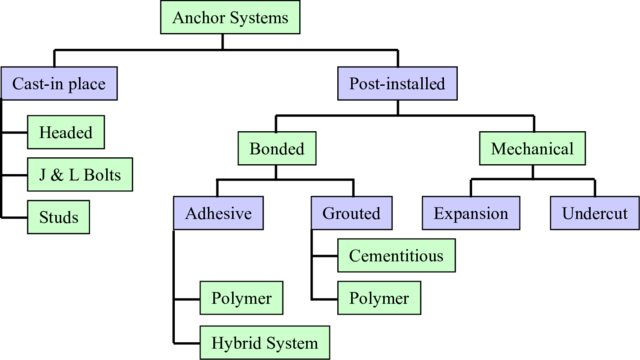
\includegraphics[width=4in]{Figures/1-Types-Anchor_system .jpg}
    \caption{Types of Anchor system}
    \cite{cook2003design}
    \label{fig:3.17}
\end{figure}
  
\subsection{Cast-in-place Anchor systems}
Anchor bolts known as "cast-in-place anchors" are fitted in wet concrete before it dries. The anchor bolt is often inserted into the foundation and sealed with wet concrete, leaving only the anchor bolt's protruding thread exposed as shown in \ref{fig:3.18}a. Figure \ref{fig:3.18} a and b shows cast-in-place anchor system. A headed steel bolt or stud shown in figure \ref{fig:3.19} is the standard component of a cast-in-place anchor. The primary method of stress transmission includes bearing on the head. Cast-in anchors have received extensive testing, and a design model has been established to precisely anticipate their behaviour \cite{cook2003design}. Cast-in-place anchor system installation is quick and follows the instructions in the dimensional drawing, which is one of the most important activities in structure design and engineering. They do not damage the concrete or require a special time and capacity.

\begin{figure}%
    \centering
    \subfloat[\centering Column-to-foundation concrete cast-in anchor system] 
    {{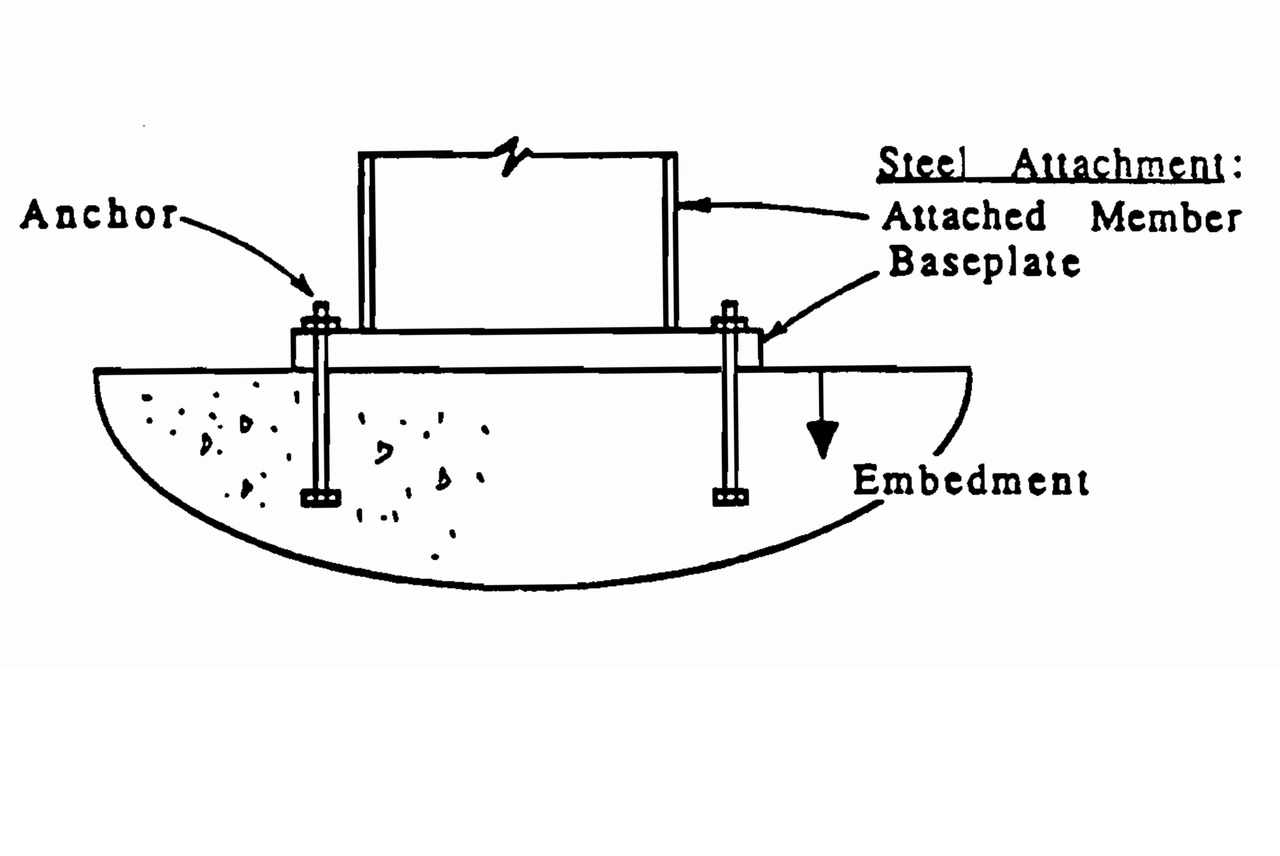
\includegraphics[width=4cm]{Figures/base_plate_image.png} }}%
     \cite{cook1989design}
    \qquad
    \subfloat[\centering Cast-in-place column-to-foundation layout plan sketch view]{{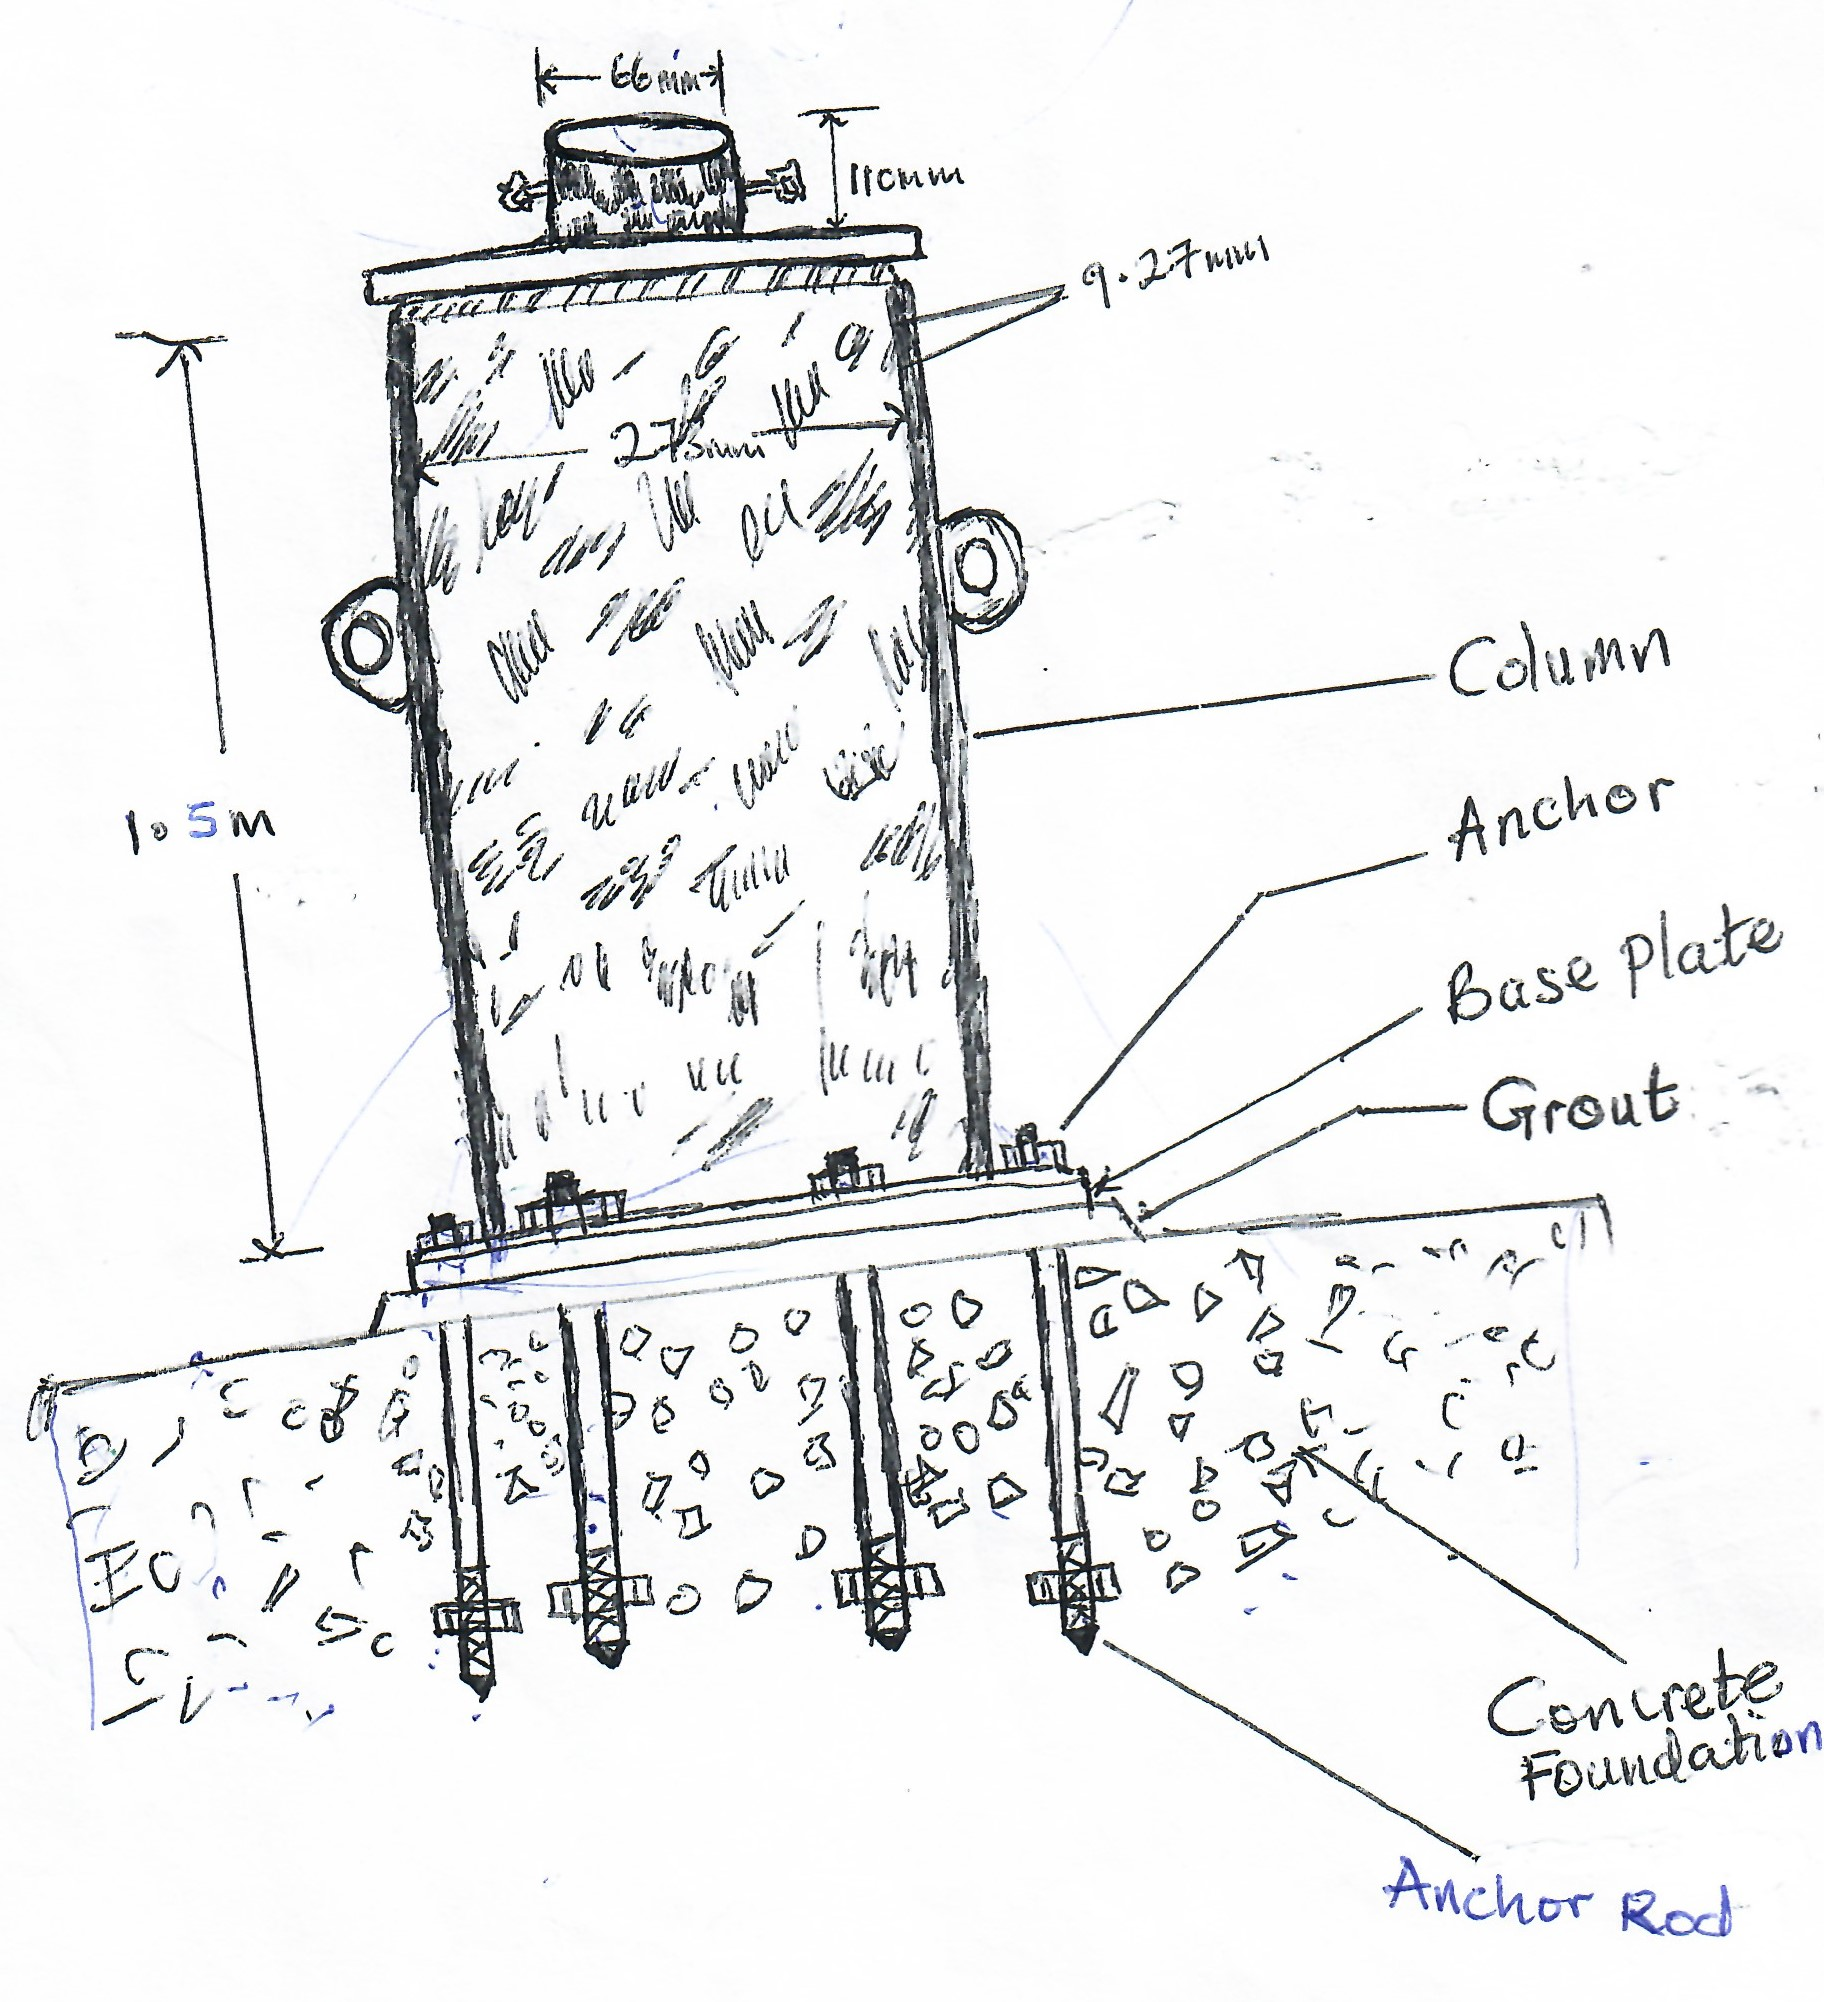
\includegraphics[width=3cm]{Figures/cast-in-anchor_design.jpg} }}%
    %\cite{doane_2016}
    \caption{Cast-in Anchor system }
    \label{fig:3.18}
\end{figure}

\begin{figure}[htp]
    \centering
    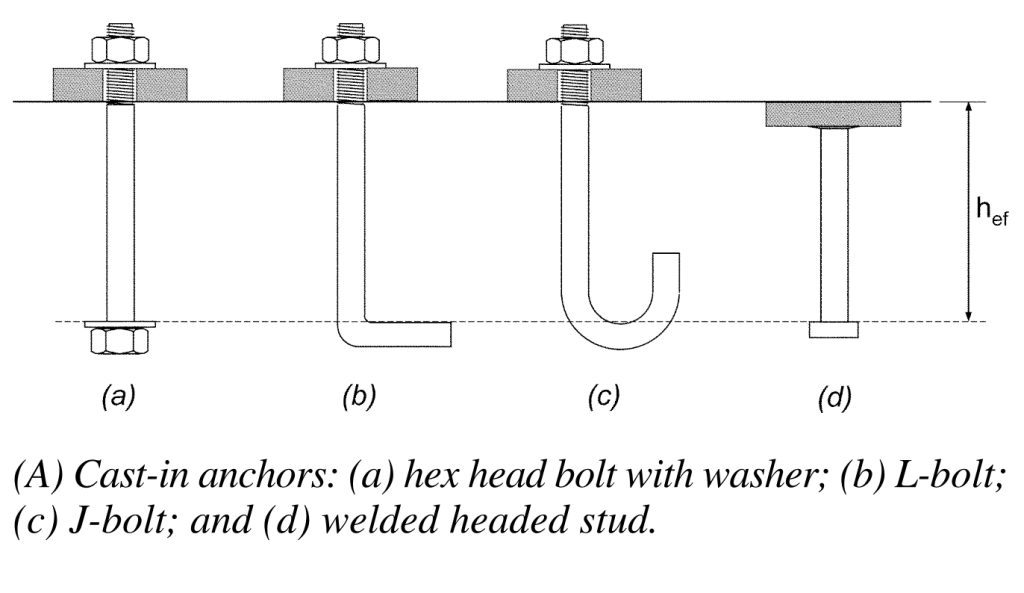
\includegraphics[width=4in]{Figures/Cast-in-anchors-1024x593.png}
    \caption{Cast-in-Anchors}
    \cite{carrato2008applying}
    \label{fig:3.19}
\end{figure}



\subsection{Design procedure of mechanical (cast-in-place) anchor bolts}

Any combination of the forces, such as tension, compression, shear, moments, and torsion, could be applied to a fastener. Individual bolts' shear and tension are the responses to these forces. As a result, the following design criteria are needed to carry out anchor bolt design against a number of possible failure modes.

\begin{enumerate}[label={}]
\item (a) Tension force resistance
\item(b) Bearing Resistance 
\item(c) Shear force resistance per shear plate
\item (d) Punching shear resistance   
\item (e)  Combined tension and shear
\end{enumerate}
The stresses on individual anchor bolts at their serviceability and ultimate limits are determined by elastic analysis below.




\subsection{F1554 grade 55 anchor bolt}

Before it was introduced as AF1554 in 1994, the ASTM F1554 specification was widely utilised around the world in several steel construction industries as A36M55, as noted by \cite{boltport2007}.
According to \cite{boltport2007}, the ASTM F1554 grade 55 anchor bolts are made of modified mild steel with a minimum yield strength of 380MPa. Anchor bolts of the F1554 grade are offered in galvanised or black finishes and additionally be able to weld.
The ASTM F1554 grade 55 anchor rods are well recognised for design circumstances where there are substantial tension pressures owing to moment connections or uplifted from overturning \cite{nand2020comparative}.
\cite{boltport2007} cites F1554 grade 55 diameters of 25.4mm with tensile strengths of 517MPa and yield strengths of 380MPa.
For low-yield carbon steel straight, headed, headless anchor bolts, bent and all-thread anchor rods, ASTM F1544 offers a range of advantages over other standard material specifications. Anchor bolts are specified with a minimum yield strength value of 55 ksi or 380 MPa in accordance with ASTM F1554 grades 36, 55, and 105. These anchor rods or anchor bolts, grade 55, are designed to secure structural supports to concrete foundations. Building columns, column supports for street signs, street lights, and traffic signals, steel bearing plates, and other similar uses are examples of such structural supports.

As part of the design process, we investigated at ASTM F1554 grade 55 for the cast-in-place anchors in the design procedure steps below.



\subsubsection{\textbf{Step 1.}}

\subsection{Tension resistance of the rod}

\textbf{Tension resistance of the rod is expressed by the formula below as:}
\begin{equation}
F_{t.Rd}=\frac{K_{2.}f_{ub}A_s}{\gamma_{M2}}
\end{equation}

\begin{enumerate}[label={}]
\item Where: 
\item \(k_2\) is a coefficient of 0.6
\item \(f_{ub}\) is the ultimate tensile strength of the rod = \(517{MP}_a\)     
\item \(A_s\) is the nominal tensile stress area of the rod = \(A_g\)
\item \(\gamma_{M2}\) is the partial safety factor of the bolt resistance = 1.25
\end{enumerate}

\textbf{Nominal tensile stress area of the rod is determined as:}
\begin{equation}
A_g = \frac{\pi d^2}{4} = \frac{\pi\times{25.4}^2}{4} = 506.7mm^2 
\end{equation}

\textbf{Tension resistance of the rod is expressed as:}
\(F_{t.Rd}=\frac{K_{2.}f_{ub}A_s}{\gamma_{M2}} = \frac{0.6\times517\times506.7}{1.25} = 125742.67M{N/mm}^2\)     

\subsubsection{\textbf{Step 2.}}


\subsection{Bearing resistance of bolts}

\textbf{Bearing resistance of the bolt is determined by the formula as follows: }
\begin{equation}
F_{b.Rd} = \frac{k_1.a_b.f_ud.t}{\gamma_{M2}}     
%\cite{fisher2006base,weynand2012resistance}
\end{equation}

\begin{enumerate}[label={}]
\item \textbf{Where:}
\item d is the nominal diameter of the rod = 25.4mm 
\item t is the thickness of the connected plate = 25mm


\item \(d_o\) is diameter of the hole direction is determined as:

\begin{equation}
d_o=d+2 = 25.4 + 2 = 27.4mm 
\end{equation} 

\item \(e_1\) is the end distance along load direction determined as:

\begin{equation}
 e_1= \geq 1.2d_{o\ }= 1.2 \times 25.4 = 32.88mm 
\end{equation}
Therefore \(e_1\) is selected to be 150mm

\item \(e_2\) is the edge distance perpendicular to load direction determined as:

\begin{equation}
 e_2 \geq 1.2d_o = 1.2\times27.4 = 32.88mm
\end{equation}
Therefore \(e_2\) is selected to be 150mm

\item \(p_1\) is the centre-to-centre spacing along load direction 

\begin{equation}
 p_1 = 2.2d_o = 2.2\times 27.4 = 60.28mm
\end{equation}

\item \(p_2\) is the centre-to-centre spacing perpendicular to load direction 
\end{enumerate}

\begin{equation}
p_2=2.4d_o = 2.4\times27.4=65.76mm
\end{equation}

\textbf{Coefficient of the  edge bolts determined by the conditions as follows:}

\textbf{condition 1}
\begin{equation}
 k_1 = (2.8\frac{e_2}{d_0}) – 1.7 = (2.8 \frac{150}{27.4}) – 1.7 = 13.62mm
\end{equation}

\textbf{condition 2}
\begin{equation}
 k_1 = (1.4\frac{p_2}{d_o}) - 1.7 = (1.4 \frac{150}{27.4}) - 1.7 = 5.96mm
\end{equation}

\textbf{condition 3}\\
\(k_1\) = 2.5mm.\\
Therefore, the inner edge bolts coefficient  \(k_1\) minimum =2.5mm

\textbf{for end bolt coefficient \(a_b\) = minimum \((a_{d }\) or \(\frac{f_{ub}}{f_u}\) or 1.9) determined below by the conditions: }      

\textbf{condition 1}
\begin{equation}
    a_d = \frac{e_1}{{3d}_o} =  \frac{150}{3\times27.4} = 1.82
\end{equation}
                    

\textbf{condition 2}
\begin{equation}
a_b = \frac{f_{ub}}{f_u} = \frac{517}{380} = 1.36 
\end{equation}
                                                              
Therefore the \(a_{b}\) minimum = 1.36 \\


\textbf{Now the bearing resistance of the bolt can be determined as:}

\(F_{b.Rd} = \frac{k_1.a_b.f_ud.t} {\gamma_{M2}} = \frac{2.5\times1.36\times380\times25.4\times25}{1.25} = 627380MN/mm^2\)




\subsection{Anchor bolt layout}

The anchor bolts' arrangement is intended to be both symmetrical in both directions and usually workable. The washer is given ample clearance from the column as a result.
 Figure \ref{fig:3.20} hole-to-hole clearance spacing  design condition by \cite{en19911} as \(e1 \geq d0\) and \(e2 \geq do\) should be met, where \(do\) is the diameter of the hole.
The minimum centre-to-centre spacing shown in  figure \ref{fig:3.20} reference must be met in accordance with the design of Steel Structures \cite{en19911} and \cite{weynand2012resistance} standards \(p1 \geq 2.2do\) and \(p2 \geq 2.4do\).




\begin{figure}
    \centering
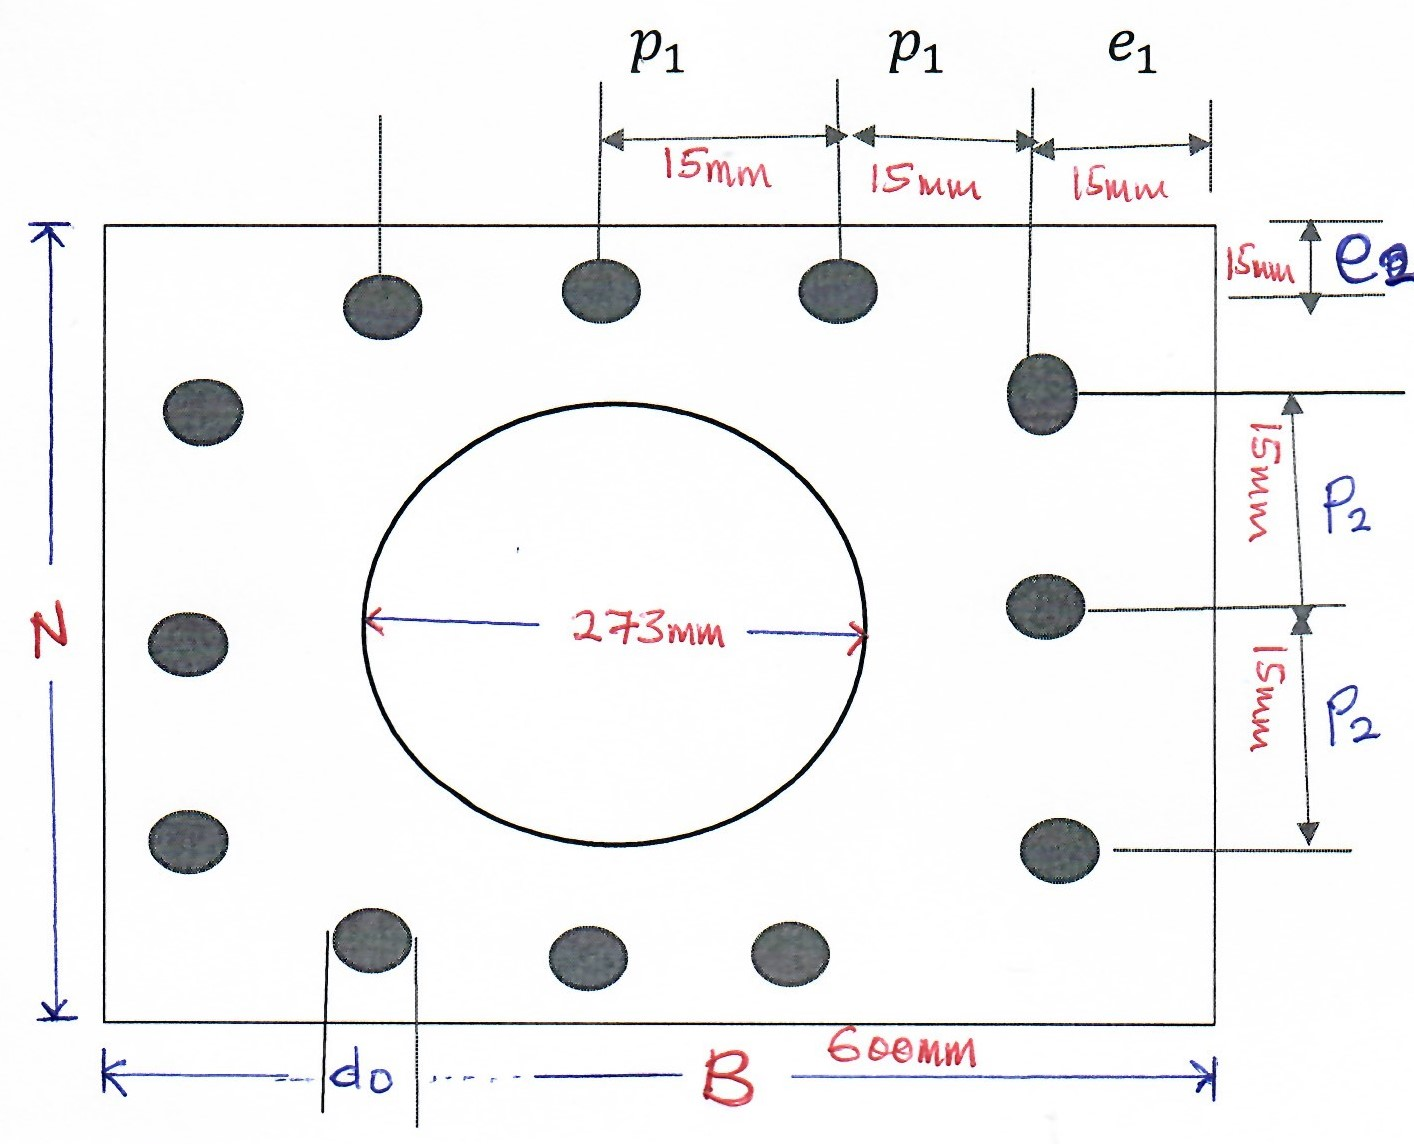
\includegraphics[width=4in]{Figures/base plate design.jpg}
\caption{Base Plate with anchor bolts layout illustration of \(P_1, P_2 centre-to-centre and e_1,e_2 edge distance \)}
 \label{fig:3.20}
\end{figure}

\subsubsection{\textbf{Step 3}}

\subsection{Shear resistance per shear plate }

\begin{equation}
    F_{vRd}=\frac{a_v. f_{ub}. A_{s}}{\gamma_{m2}} = \frac{{0}.{6}\times{517}\times{1134}}{{1}.{25}}=281413.4MN/m{m}^{2}
\end{equation}


\subsubsection{\textbf{Step 4}}

\subsection{Punching strength of the bolt}


\begin{equation}
 B_{p.Rd} = \frac{0.6.\pi d_m.t_{p}.f_u}{\gamma_{M2}} =  \frac{0.6\times \pi \times38\times380}{1.25} = 21775MN/mm^2
\end{equation}

 Where: \(d_m\) is the mean of the cross point and across flats dimension of the bolts head.
 

\subsubsection{\textbf{Step 5}}

\subsection{Combined shear and Tension}
Anchor bolts that are subjected to both axial tension and shear must satisfy the very same unity equation as anchor bolts that are designed for allowable stress:
\cite{NCMA2022} specifies the appropriate strength reduction factors to be used, which are \(\Phi\) = 0.5 for masonry crushing under shear loads and \(\Phi\) = 0.9 for anchor yielding under tensile stresses.


\begin{equation}
\frac{{ F}_{{vEd}}}{{\phi F}_{{vRd}}}+\frac{{F}_{{tEd}}}{\Phi{F}_{{tRd}}} \le{1}
= \frac{{380}}{{ 0.9 \times 281413}.{4}}+\frac{{517}}{{0}.{5}\times{281413}.{44}} <{1} = 0.0052 <{1}
\end{equation}

\textbf{Since the demand combined shear and tension capacity ratio is less than 1.0, the anchor bolt design is therefore satisfactory.}




\section{Concrete Footing Foundation Design}


The portion of a structure known as the foundation often rests below the surface of the ground and transfers load to the soil or rock beneath. When loaded, all soils significantly compress, which causes the supporting structure to move.
The load of the structure must be (1) transmitted to a soil stratum with adequate strength, and (2) distributed across a sufficient area of that stratum to minimise bearing pressure, in order to prevent settlements as stated.
In order for a concrete structure to serve the purpose for which it was constructed and safely withstand the factors that will impact on it during its useful life, the general shape and precise specifications must be determined \cite{darwin2016design}. The main factors affecting it will be the loads and other forces to which it will be subjected, along with other unfavourable elements including wind loads, temperature changes, and foundation settlements. The intended purpose of the building determines its fundamental design.
There are four main types of shallow footing foundations: there are combination footing, strip footing, raft footing foundation, and pad footing. For the specification of our design, we will focus on the pad footing foundation.

\subsection{Pad foundation}
Pad foundations are circular or rectangular pads that support just a small area of weight, such as a single column. They are more prevalent on bigger, specifically designed buildings like industrial units or other commercial constructions to support big roofed structures. Example of pad footing foundation with the footing design parameters is shown in Figure \ref{fig:3.21}.


\begin{figure}
    \centering
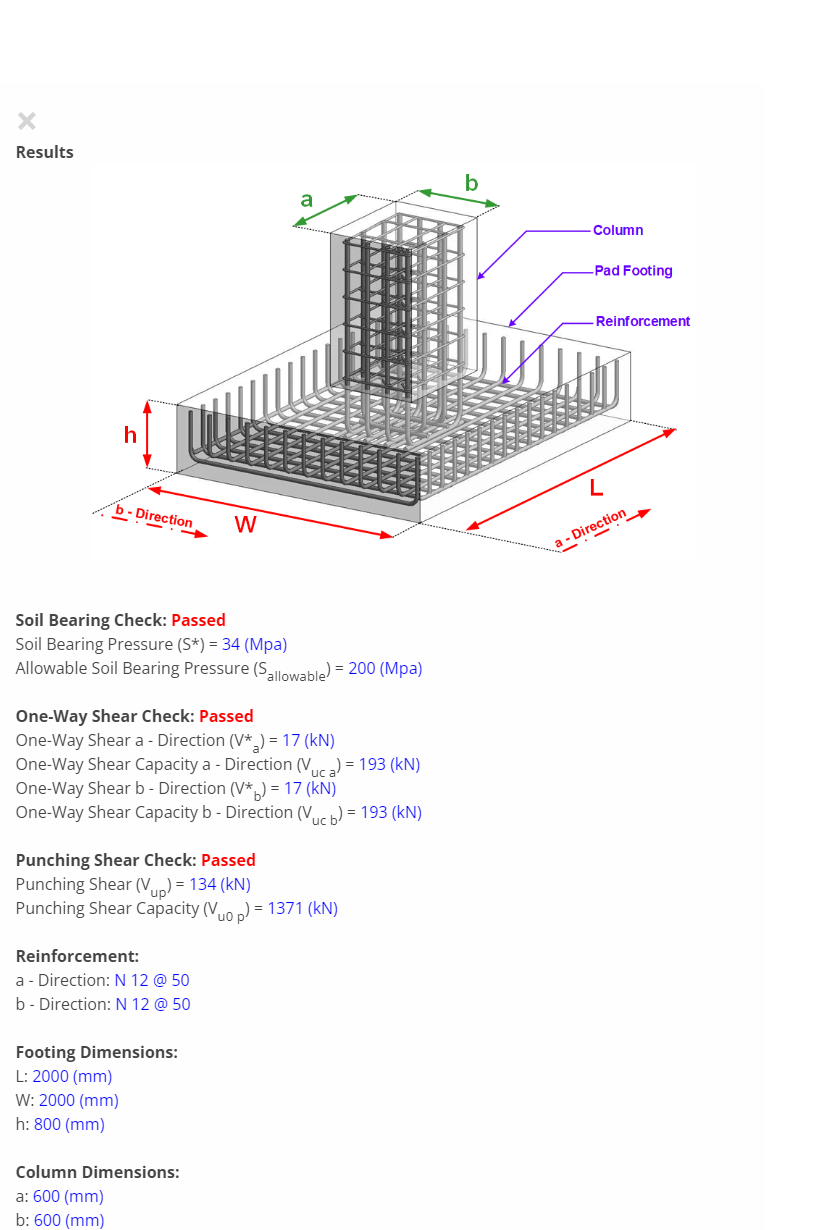
\includegraphics[width=6in]{Figures/tap foundation design2.png}
\caption{Concrete column Pad footing foundation with the design parameters}
 \label{fig:3.21}
\end{figure}



\section{Summary}

Taken into consideration the Mauritian cyclonic weather, the chapter emphases on the mechanical and the structural design of the system to be able to withstand the condition. Methods for the instrument's safety and optimisation were given, and the overall architecture was assessed. The authors' goal is to design each component of the antenna structure system to bear loads or pressures from both the internal and external loads.

The wind load parameters were investigated using practical and standard recommended methodologies, taking into account the site's location. Additionally, a calculation was made to determine the anticipated wind stress on the 2.4m parabolic dish's surface. The results are summarised in table  \ref{tab:3.6}, \ref{tab:3.7} and \ref{tab:3.8} of the design.


\begin{table}[h!]
    \centering

\caption{\textbf{Summary of the antenna column design parameters}}

\begin{tabular}{ c   c}
    \hline
 
 Parabolic dish diameter & 2.4m\\ 

 Antenna column diameter & 273mm \\

 Moment of force & 15.35kN\\


 Column deflection  &  0.0032m\\

Column weight & 90.8kg/m\\
 \hline
 
    \end{tabular}
    \label{tab:3.6}
\end{table}

\vspace{1cm}
 
 \begin{table}[h!]
    \centering
 
  \caption{\textbf{Summary of the antenna base plate design parameters}}
\begin{tabular}{ c  c}
    \hline
 Base plate diameter & 0.6m x 0.6m\\

Type of welding joint & circular fillet\\

Shear stress of the weld joint & 117.6MPa\\

Welded joint SoF & 8.97\\

Anchor bolt system & cast-in-place\\

Anchor bolt type & F1554 grade 55\\

Bolt length & 100mm\\

Bolt diameter & 27.4mm\\

Bolt layout spacing & 150mm\\

Punching strength of the bolt & 21775MN/\(mm^2\)\\

Combined shear and tension capacity & 0.0052\\
\hline
 \end{tabular}
    \label{tab:3.7}
\end{table}

The techniques and welding optimisation were also followed to choose and establish the ideal welding joint and stress for the antenna. A successful determination of the allowed fatigue stress and the factor of safety was achieved.



 \begin{table}[h!]
    \centering
 
  \caption{\textbf{Summary of the antenna concrete footing foundation design parameters}}
\begin{tabular}{ c c }
    \hline
Concrete footing foundation & Pad footing\\ 

Soil bearing capacity & 34MPa \\

Allowable soil bearing capacity & 200MPa \\

Concrete footing pouncing shear & 134kN \\

Concrete punching shear capacity & 1371kN\\

Footing length & 2000mm\\

Footing width & 200mm\\

Footing height & 800mm\\
\hline

    \end{tabular}
    \label{tab:3.8}
\end{table}

The procedure involves designing and anchoring the antenna column and the structural system in order to support the antenna and protect it from external forces like wind loads, which were investigated and followed. The design conditions say that both the tension capacity ratio and the bearing resistance of the bolt should be less than 1.0, which satisfies the design condition. Last but not least, the concrete footing foundation was designed so that loads from the structure could be easily transferred to the soil.
In the next chapter, we'll talk about the parameter simulation test and result analysis that were done using SolidWorks software.












}